%\documentclass[notes]{beamer}       % print frame + notes
%\documentclass[notes=only]{beamer}   % only notes
\documentclass{beamer}              % only frames

\usepackage{pgfpages}

% \setbeamertemplate{note page}[plain]
% \setbeameroption{show notes on second screen}

\usepackage{amsmath, amssymb, float, amsthm}
\usepackage{fancyvrb}

\usepackage{amsfonts}

\usepackage{hyperref}

%\usepackage{verbatim}

% row color
\usepackage{color, colortbl}
\definecolor{LightCyan}{rgb}{0.88,1,1}

\newcolumntype{a}{>{\columncolor{LightCyan}}r}

\usepackage{booktabs}
\usepackage{tabularx}
\usepackage{parcolumns}
\usepackage{listings}

\usepackage{graphics}
\usepackage{graphicx,multirow}
\usepackage{epsfig}

% strikeout text
\usepackage{ulem}

% footnote size
\setbeamerfont{footnote}{size=\scriptsize}

% drawing Petri nets
\usepackage{tikz}
\usetikzlibrary{arrows,shapes,automata,petri,positioning}

\tikzset{
    place/.style={
        circle,
        thick,
        draw=blue!75,
        fill=blue!20,
        minimum size=6mm,
    },
    transitionH/.style={
        rectangle,
        thick,
        fill=black,
        minimum width=8mm,
        inner ysep=2pt
    },
    transitionV/.style={
        rectangle,
        thick,
        fill=black,
        minimum height=8mm,
        inner xsep=2pt
    }
}

% draw hierarchy tree
\usepackage{forest}
\usepackage{tikz-qtree}

\newcommand{\blue}[1]{\textcolor{blue}{#1}}
\newcommand{\red}[1]{\textcolor{red}{#1}}

\usetheme[secheader]{Boadilla}

\title{New ideas for scalable attractor detection and control of asynchronous Boolean networks}
\author[Van-Giang Trinh]{Van-Giang Trinh\inst{1}, Samuel Pastva\inst{2}, Kyu Hyong Park\inst{3} and Jordan Rozum\inst{4}}

\date{\today}
%\date{July 13, 2022}

\institute[] % (optional, but mostly needed)
{
  \inst{1}
  LIS, Aix-Marseille University, France
  
  \inst{2}
  Institute of Science and Technology, Austria
  
  \inst{3}
  Pennsylvania State University, United States of America
  
  \inst{4}
  Binghamton University, United States of America
}

% \AtBeginSection[] {
%   \begin{frame}
%     \frametitle{Contents}
%     \tableofcontents[currentsection]  
%   \end{frame}
% }

% \AtBeginSubsection[] {
%   \begin{frame}
%     \frametitle{Outline}
%     \tableofcontents[currentsection, currentsubsection]  
%   \end{frame}
% }

% \makeatletter
% \def\beamer@setupnote{%
%   \gdef\beamer@notesactions{%
%     \beamer@outsideframenote{%
%       \beamer@atbeginnote%
%       \beamer@notes%
%       \ifx\beamer@noteitems\@empty\else
%       \begin{itemize}\itemsep=0pt\parskip=0pt%
%         \beamer@noteitems%
%       \end{itemize}%
%       \fi%
%       \beamer@atendnote%
%     }%
%     \gdef\beamer@notesactions{}%
%   }
% }
% \makeatother

\begin{document}

\begin{frame}
  \titlepage
\end{frame}

\begin{frame}
  \frametitle{Attractor detection and control of asynchronous Boolean networks}

Two \blue{most important} issues in Boolean networks research with many applications in various fields~\cite{akutsu2018algorithms, schwab2020concepts}.

\hspace{0.8cm}

Usually, the attractor detection issue is the preceding step of the control issue.

\hspace{0.8cm}

Unfortunately, both of them are \red{very challenging}, especially for \red{large-scale} networks.

\hspace{0.8cm}

Many methods have been proposed.

\end{frame}

\begin{frame}
  \frametitle{Attractor detection methods}

BDD-based methods: genYsis~\cite{DBLP:journals/bioinformatics/GargCXMM08}, geneFatt~\cite{zheng2013efficient}, \blue{CABEAN}~\cite{DBLP:journals/tcbb/MizeraP0Y19, DBLP:conf/fm/SuP21}.

\hspace{0.8cm}

Reduction-based methods: \blue{AEON}~\cite{DBLP:conf/cav/BenesBPS21}.

\hspace{0.8cm}

Trap space-based methods: PyBoolNet~\footnote{It is not an exact method.}~\cite{klarner2017pyboolnet}, \blue{pystablemotifs}~\cite{Rozum2021, rozum2021pystablemotifs}.

\hspace{0.8cm}

Feedback vertex set-based methods: FVS-ABN~\cite{GiangTCBB2020}, iFVS-ABN~\cite{DBLP:conf/cibcb/GiangH21}, \blue{mtsNFVS}~\cite{DBLP:conf/bcb/TrinhHB22}.

\hspace{0.8cm}

All of them have \blue{advantages} and \red{disadvantages}.
To our best knowledge, none of them can robustly handle \red{complex networks with thousands of nodes}.

\end{frame}

\begin{frame}
  \frametitle{Control methods}

BDD-based and decomposition-based methods: \blue{CABEAN}~\cite{DBLP:journals/bioinformatics/SuP21, DBLP:conf/fm/SuP21}.

\hspace{0.8cm}

Reduction-based methods: \blue{AEON}~\cite{Brim2021}.

\hspace{0.8cm}

Trap space-based methods: PyBoolNet~\cite{cifuentes2020control, cifuentes2021control}, \blue{pystablemotifs}~\cite{Zaudo2015, rozum2021pystablemotifs}.

\end{frame}

\begin{frame}
\frametitle{Objective}

pystablemotifs and mtsNFVS have \blue{much more potential} to reach the \red{genome scale}.

\hspace{0.8cm}

Both of them have their own advantages and disadvantages, but fortunately they can be \blue{complementary} to each other.

\hspace{0.8cm}

Develop a \blue{more efficient method} that can benefit both the attractor detection and control issues, and in particular can handle networks at the genome scale.
    
\end{frame}

\begin{frame}
  \frametitle{pystablemotifs}

\centering
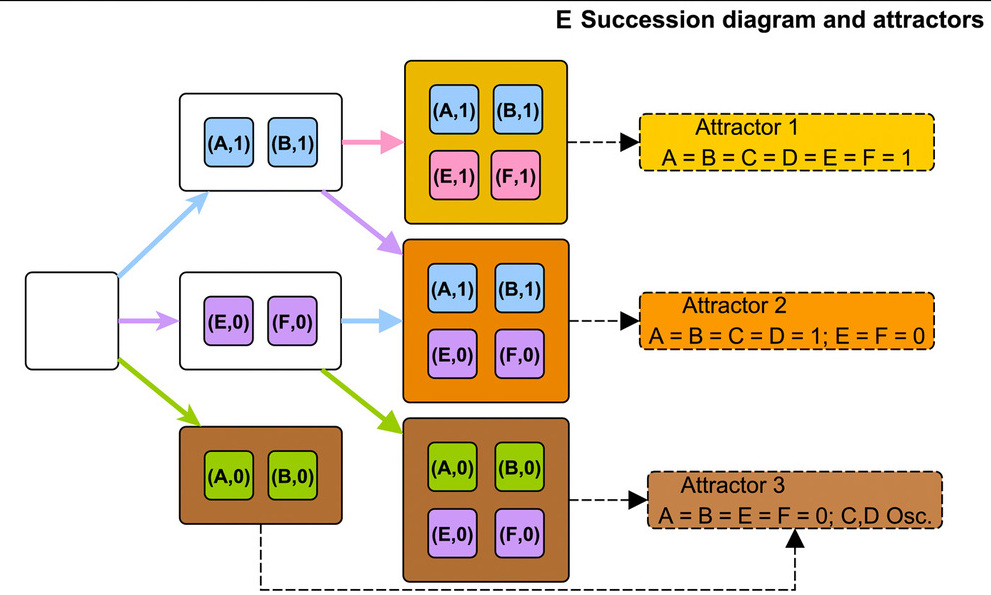
\includegraphics[scale=0.3]{Figures/succession_diagram.jpg}

\begin{tikzpicture}[remember picture, overlay]
  \only<2>{\node[below=-0.6cm of current page.west, blue, fill=green!10, xshift=6cm, text width=0.8\textwidth] (a-2) {- stable motif = maximal trap space\\- "quasi" attractor = minimal trap space\\- motif-avoidant attractor = ?};}
  
  \only<3>{\node[below=-0.6cm of current page.west, blue, fill=green!10, xshift=6cm, text width=0.8\textwidth] (a-3) {- pystablemotifs is beneficial to not only the attractor detection problem but also the control problem as it provides a \red{succession diagram} that can be efficiently used for control.\\- If solely considering attractor identification, pystablemotifs seems to have \red{disadvantages} as compared to other methods such as AEON, iFVS-ABN, and mtsNFVS.};}
  
  \only<4>{\node[below=-0.6cm of current page.west, blue, fill=green!10, xshift=6cm, text width=0.8\textwidth] (a-4) {- pystablemotifs must check the existence of \red{motif-avoidant attractors}.\\- Although it uses time reversal to prune the considered state space, the remaining part (called the terminal restriction space) may be still \red{too large} to be analyzed.};}
  
  \only<5>{\node[below=-0.6cm of current page.west, blue, fill=green!10, xshift=6cm, text width=0.8\textwidth] (a-5) {- pystablemotifs relies on PyBoolNet to compute stable motifs (i.e., maximal trap spaces). However, PyBoolNet does not work well with networks with Boolean functions having many input nodes.\\- The reason for this is PyBoolNet mainly relies on prime-implicants computation, whereas the number of prime-implicants may be too huge if there are many input nodes.};}
  
  \only<6>{\node[below=-0.6cm of current page.west, blue, fill=green!10, xshift=6cm, text width=0.8\textwidth] (a-6) {- The size of the succession diagram may be too large.\\- Apart from the theoretical worst case (\(n_{sm}!\) where \(n_{sm}\) is the number of stable motifs), the number of stable motifs may be actually too large because for example, the network has two many source nodes (node \(A\) is a source node if \(f_A = A\)).};}
\end{tikzpicture}

\end{frame}

\begin{frame}
  \frametitle{mtsNFVS}

\centering
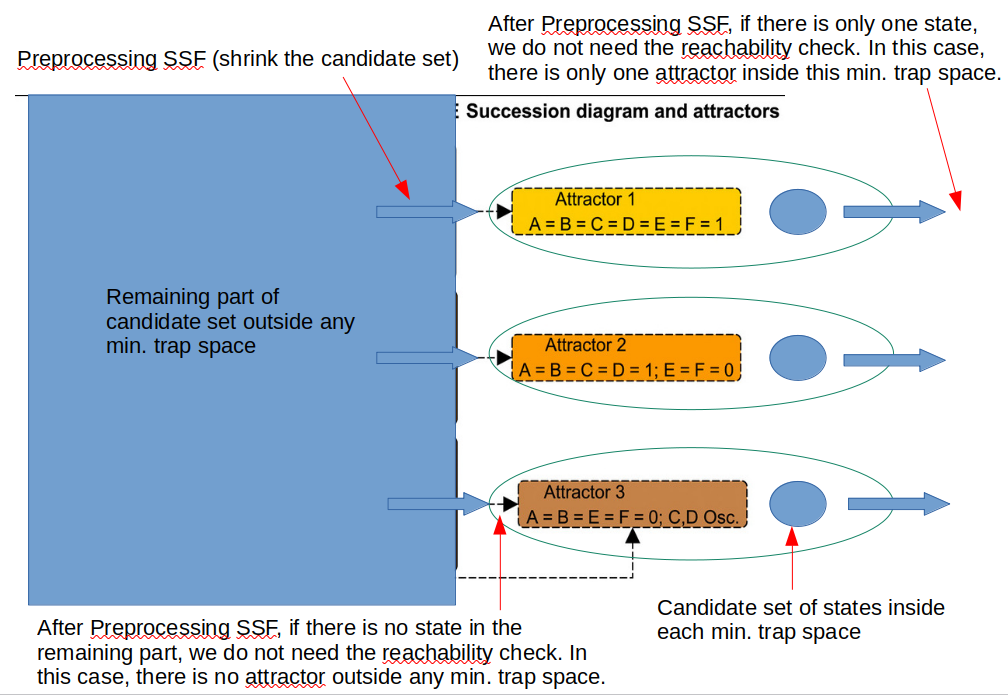
\includegraphics[scale=0.3]{Figures/mtsNFVS.png}

\begin{tikzpicture}[remember picture, overlay]
  \only<2>{\node[below=-0.6cm of current page.west, blue, fill=green!10, xshift=6cm, text width=0.8\textwidth] (a-2) {- The candidate set \(F\) (the blue part) is computed based on an negative feedback vertex set \(U^{-}\) of the ABN.};}
  
  \only<3>{\node[below=-0.6cm of current page.west, blue, fill=green!10, xshift=6cm, text width=0.8\textwidth] (a-3) {- If the size of the negative feedback vertex set is too large, there may be too many states in the candidate set \(F\) (i.e., the set of fixed points of the reduced STG), leading to extremely longer time for the computation of \(F\), Preprocessing SSF, and maybe the reachability analysis.\\- Note that real-world models usually have \red{small} minimum negative feedback vertex sets.};}
  
  \only<4>{\node[below=-0.6cm of current page.west, blue, fill=green!10, xshift=6cm, text width=0.8\textwidth] (a-4) {- mtsNFVS also uses PyBoolNet to compute the candidate set as well as the set of minimal trap spaces. Again, it will not work well with the case of many input nodes.};}
  
  \only<5>{\node[below=-0.6cm of current page.west, blue, fill=green!10, xshift=6cm, text width=0.8\textwidth] (a-5) {- If some motif-avoidant attractors exist or the results of Preprocessing SSF are not good enough, mtsNFVS still must check the reachability in asynchronous BNs, which is PSPACE-complete in general.\\- Moreover, the target set for the reachability analysis is maybe small (i.e., the union of all minimal trap spaces).};}
  
  \only<6>{\node[below=-0.6cm of current page.west, blue, fill=green!10, xshift=6cm, text width=0.8\textwidth] (a-6) {- Currently, mtsNFVS focuses solely on the attractor detection problem.};}
\end{tikzpicture}

\end{frame}

\begin{frame}
  \frametitle{New idea}

In principle, our new idea is to combine pystablemotifs and mtsNFVS to obtain a more efficient method that can benefit both the attractor detection and control problems.

\hspace{0.8cm}

Hereafter, we will present the general approach along with many \blue{new findings} that can speedup the whole process.

\end{frame}

\begin{frame}
  \frametitle{General approach}

\only<1>{\red{It follows the process of pystablemotifs (i.e., building the succession diagram)}.}

\centering
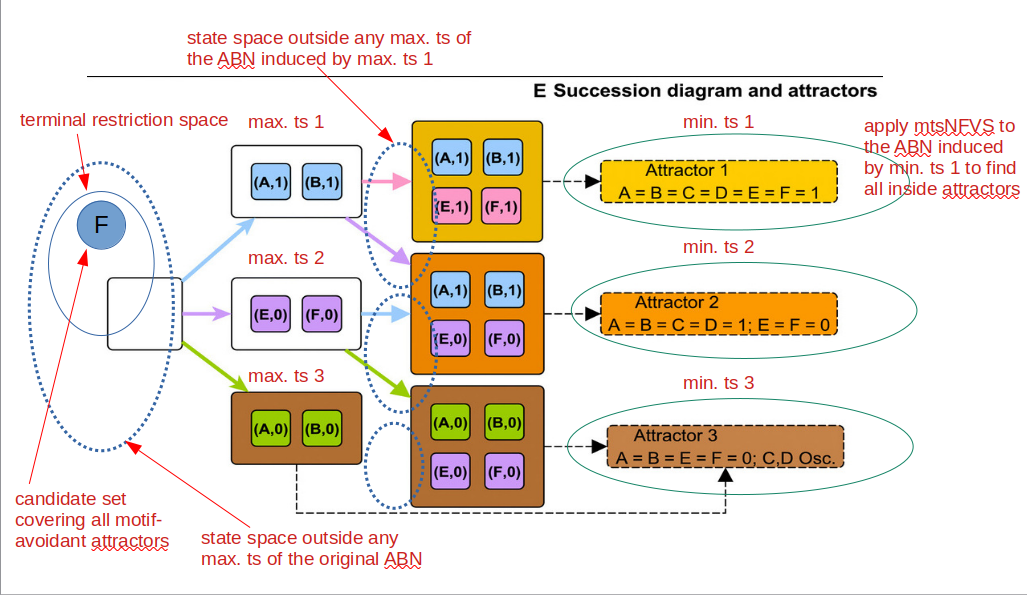
\includegraphics[scale=0.33]{Figures/general_approach.png}

\begin{tikzpicture}[remember picture, overlay]
  \only<2>{\node[below=-3.0cm of current page.center, blue, fill=green!10, xshift=2.2cm, text width=0.65\textwidth] (a-2) {- We need to check the existence of motif-avoidant attractors.\\- We compute the terminal restriction space \(R\).\\- We compute the candidate set \(F\) covering all motif-avoidant attractors. Each state in \(F\) must be in \(R\) and has no out-going successor after systematically removing some of its successors according to the negative feedback vertex set of the original ABN.\\- \(F\) may be \red{small} even when the NFVS is large.};}
  
  \only<3>{\node[below=-3.0cm of current page.center, blue, fill=green!10, xshift=2.2cm, text width=0.65\textwidth] (a-3) {\small - Next, we use Preprocessing SSF for \(F\) with the target set \(M_{max}\) of states covered by the union of all max. trap spaces of the original ABN. \\- If Preprocessing SSF is good enough, we can reach the \red{best} case where \(F = \emptyset\) (i.e., there is no motif-avoidant attractor outside the max. trap spaces).\\- Otherwise, we need to check the reachability with the target set including \(M_{max}\).\\- \red{Computation of \(\Delta\) is not demanding. Let \(S_{\Delta}\) be the set of states induced by \(\Delta\). We can use \(S_{\Delta} \cup M_{max}\) instead of only \(M_{max}\)}.};}
  
  \only<4>{\node[below=-3.0cm of current page.center, blue, fill=green!10, xshift=3cm, text width=0.5\textwidth] (a-3) {- We repeat the above process for the ABNs induced by max. trap spaces 1, 2, 3, ... along with building the succession diagram\\- Note that the induced ABNs may be much smaller and simpler than the original ABN, leading to the significant reduction in the size of the NFVS.};}
  
  \only<5>{\node[below=-0.6cm of current page.west, blue, fill=green!10, xshift=3.5cm, text width=0.55\textwidth] (a-5) {- Finally, we need to compute all attractors inside each min. trap space.\\- We can simply apply the approach of mtsNFVS to the ABN induced by the min. trap space.};}
  
  \only<6>{\node[below=-0.6cm of current page.west, blue, fill=green!10, xshift=6cm, text width=0.8\textwidth] (a-6) {- One natural question is that why not directly perform the motif-avoidant attractor checking for the original ABN with the set of min. trap spaces?.\\- What are other benefits apart from obtaining the succession diagram that is then used for control?};}
  
  \only<7>{\node[below=-0.6cm of current page.west, blue, fill=green!10, xshift=6cm, text width=0.8\textwidth] (a-7) {- First, the new approach of course obtains not only the set of attractors but also the succession diagram that is then used for control.\\- Second, we observed that in this case the terminal restriction space may be \red{too huge}, leading to the candidate set \(F\) may be too large (hence, hard to be computed as well).\\- Third, \(M_{max}\) is much broader than \(M_{min}\) in most cases, hence using max. trap spaces can help Preprocessing SSF to reach good cases \red{more easily} than using min. trap spaces.};}
  
  \only<8>{\node[below=0.0cm of current page.center, blue, fill=green!10, xshift=0cm, text width=1\textwidth] (a-8) {Jordan: We need to consider the percolation of a stable motif (LDOI) along with building the succession diagram. The percolation is based on PyBoolNet.\\Sam: When we have already obtained the stable motif (i.e., max. trap space), we can perform the percolation easily by algebraically propagating the fixed values.\\Giang: Sure. It is possible. Note that we can store Boolean functions as Boolean expressions or BDDs (not as prime-implicants).};}
  
\end{tikzpicture}

\end{frame}

\begin{frame}
  \frametitle{Network reduction}

\centering
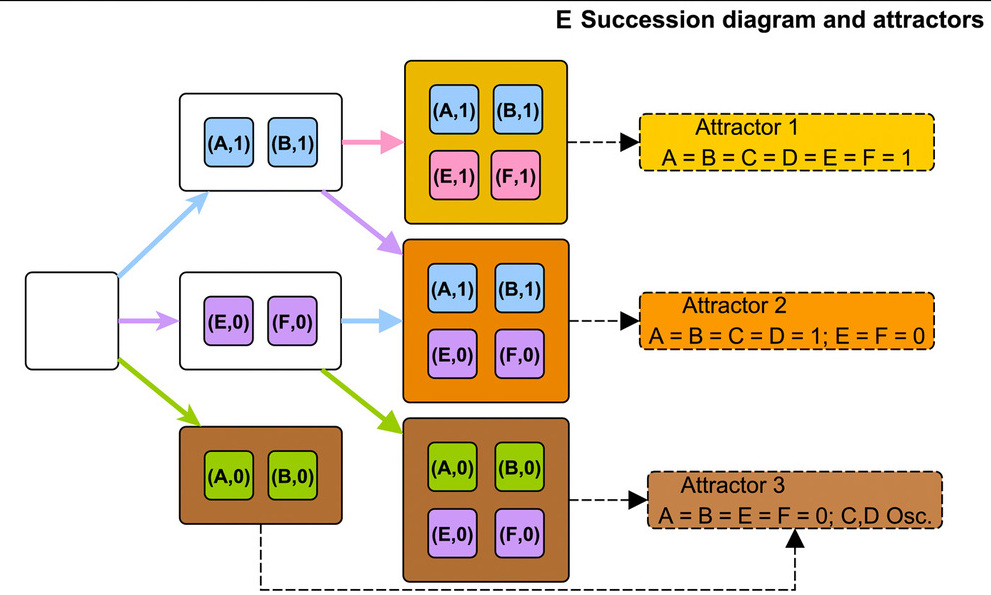
\includegraphics[scale=0.33]{Figures/succession_diagram.jpg}

\begin{tikzpicture}[remember picture, overlay]
  \only<1>{\node[below=-3.0cm of current page.center, blue, fill=green!10, xshift=2.2cm, text width=0.65\textwidth] (a-1) {- There are some reduction techniques for Boolean networks that preserve attractors and trap spaces.\\- \red{leaf-node reduction}~\cite{DBLP:conf/cmsb/NaldiMC12}\\- constant-node and intermediate-node reduction~\cite{DBLP:journals/siamads/SaadatpourAR13}};}
  
  \only<2>{\node[below=-3.0cm of current page.center, blue, fill=green!10, xshift=2.2cm, text width=0.65\textwidth] (a-2) {- First, we can apply our whole method to the BN \(\mathcal{N}^{re}\) obtained by applying the leaf-node reduction to the original BN \(\mathcal{N}\).\\- From the results (attractors, min. trap spaces) on \(\mathcal{N}^{re}\) we can easily derive the results on \(\mathcal{N}\).};}
  
  \only<3>{\node[below=0cm of current page.center, blue, fill=green!10, xshift=2.2cm, text width=0.65\textwidth] (a-3) {- Second, in each \red{intermediate BN} \(N\) induced by \textbf{previous} max. trap spaces, we can apply the leaf-node reduction in the computation of \textbf{current} max. trap spaces.\\- Let \(N^{red}\) be the reduced BN. By using siphons, we can easily prove that a max. trap space of \(N^{red}\) is exactly a max. trap space of \(N\) without projection.};}
  
  \only<4>{\node[below=0cm of current page.center, blue, fill=green!10, xshift=2.2cm, text width=0.65\textwidth] (a-4) {Other applications of network reduction techniques to our method?};}
  
\end{tikzpicture}

\end{frame}

\begin{frame}
  \frametitle{Deal with the problem of large succession diagrams}

\only<1>{\red{The above approach is promising. However, how to deal with the problem of large succession diagrams?}.}

\centering
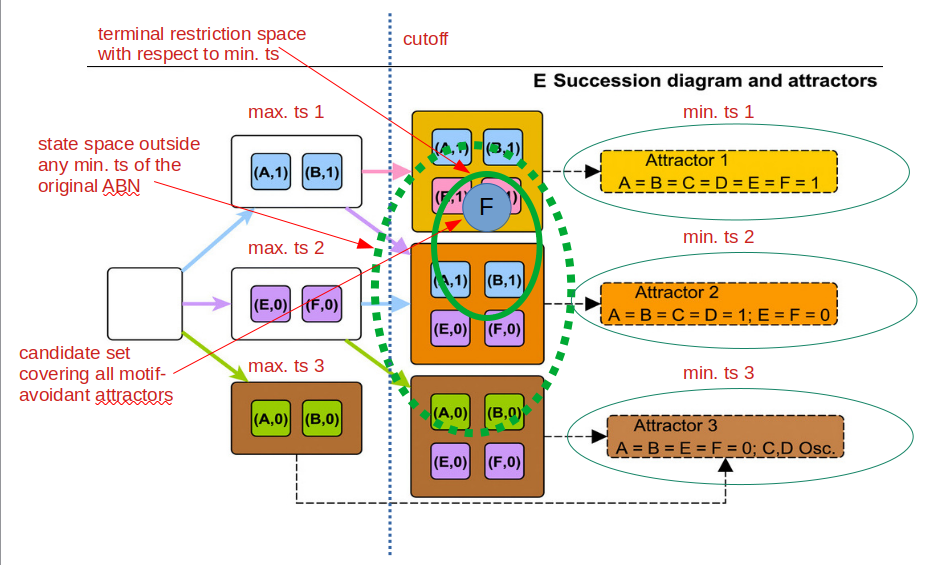
\includegraphics[scale=0.33]{Figures/deal_with_large_sd.png}

\begin{tikzpicture}[remember picture, overlay]
  \only<2>{\node[below=2.0cm of current page.center, blue, fill=green!10, xshift=0cm, text width=0.9\textwidth] (a-2) {- When the size of the succession diagram becomes too large (maybe exceeding a threshold), we stop its construction.\\- However, we still need to check the existence of motif-avoidant attractors.};}
  
  \only<3>{\node[below=2.0cm of current page.center, blue, fill=green!10, xshift=0cm, text width=1\textwidth] (a-3) {\small - First, we compute all min. trap spaces of the original ABN.\\- Second, we compute the terminal restriction space \(R\) with respect to these min. trap spaces.\\- Next, we get the intersection between \(R\) and the state spaces induced by the already computed max. trap spaces \red{and their LDOIs} (e.g., max. ts 1, 2, 3). };}
  
  \only<4>{\node[below=2.0cm of current page.center, blue, fill=green!10, xshift=0cm, text width=1\textwidth] (a-4) {- Then, we compute the candidate set \(F\) with respect to the NFVS of the original ABN.\\- Each state in \(F\) must be in the intersected set obtained beforehand.\\- \(F\) may be \red{small} even when the NFVS is large because the intersected set may be not too large.};}
  
  \only<5>{\node[below=1.5cm of current page.center, blue, fill=green!10, xshift=0cm, text width=1\textwidth] (a-5) {Next, we use Preprocessing SSF for \(F\) with the target set \(M_{min}\) of states covered by the union of all min. trap spaces of the original ABN. \\- If Preprocessing SSF is good enough, we can reach the best case where \(F = \emptyset\) (i.e., there is no motif-avoidant attractor).\\- Otherwise, we need to check the reachability with the target set including \(M_{min}\).};}

  \only<6>{\node[below=2.5cm of current page.center, blue, fill=green!10, xshift=0cm, text width=1\textwidth] (a-6) {- Finally, we need to compute all attractors inside each min. trap space.\\- We can simply apply the approach of mtsNFVS to the ABN induced by the min. trap space.};}
  
  \only<7>{\node[below=2.5cm of current page.center, blue, fill=green!10, xshift=0cm, text width=1\textwidth] (a-7) {- After finishing the above process, we will obtain the whole attractor landscape and the partial succession diagram.};}
\end{tikzpicture}

\end{frame}

\begin{frame}
  \frametitle{Computation of max. trap spaces}

\centering
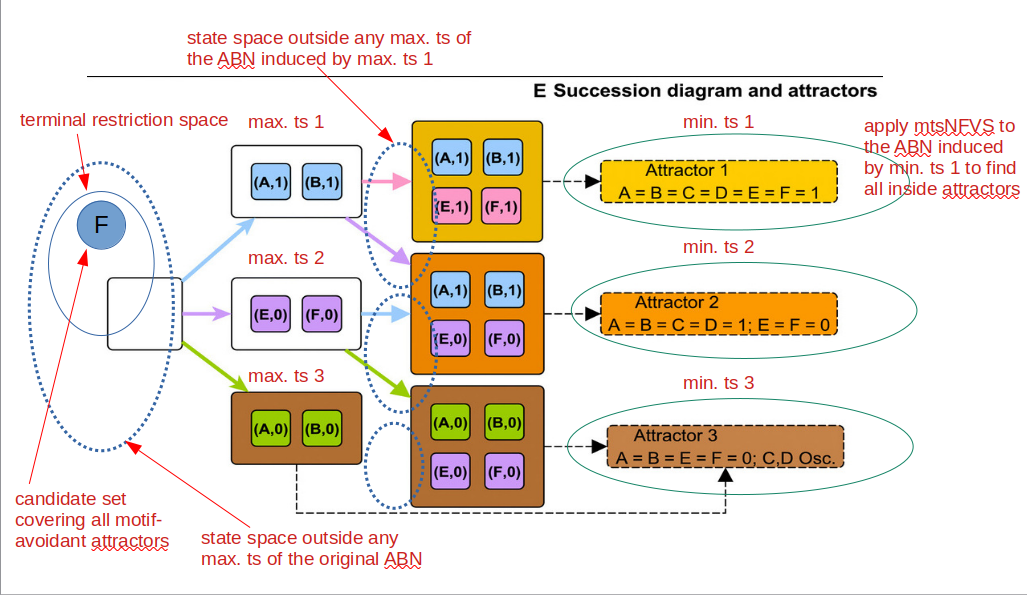
\includegraphics[scale=0.33]{Figures/general_approach.png}

\begin{tikzpicture}[remember picture, overlay]
  \only<1>{\node[below=-3.0cm of current page.center, blue, fill=green!10, xshift=2.2cm, text width=0.65\textwidth] (a-1) {- pystablemotifs uses PyBoolNet to compute max. trap spaces.\\- The bottleneck of PyBoolNet is the huge number of prime-implicants.\\- We need a \red{more efficient} method for computing max. trap spaces.};}
  
  \only<2>{\node[below=-3.0cm of current page.center, blue, fill=green!10, xshift=2.2cm, text width=0.65\textwidth] (a-2) {- Fortunately, we have already had one.\\- Recently, we have proposed a new method called Trappist for computing minimal trap spaces of Boolean networks~\cite{DBLP:conf/cmsb/TrinhBHS22}.\\- Trappist completely outperforms PyBoolNet and it can \red{tame} the case of many input nodes. In particular, it can handle networks of the \red{genome scale}.};}
  
  \only<3>{\node[below=-3.0cm of current page.center, blue, fill=green!10, xshift=2.2cm, text width=0.65\textwidth] (a-3) {- In~\cite{DBLP:conf/cmsb/TrinhBHS22}, we have proved that a trap space of a BN is equivalent to a conflict-free siphon of its Petri net encoding.\\- Consequently, a min. trap space is equivalent to a maximal conflict-free siphon. Trappist computes min. trap spaces by computing maximal conflict-free siphons.\\- We can easily prove that a \red{max. trap space} is equivalent to a \red{minimal conflict-free siphon}.\\- Now, Trappist does not support computing max. trap spaces. However, we can easily develop this feature for Trappist.};}
\end{tikzpicture}

\end{frame}

\begin{frame}
\frametitle{Computation of terminal restriction spaces}

\centering
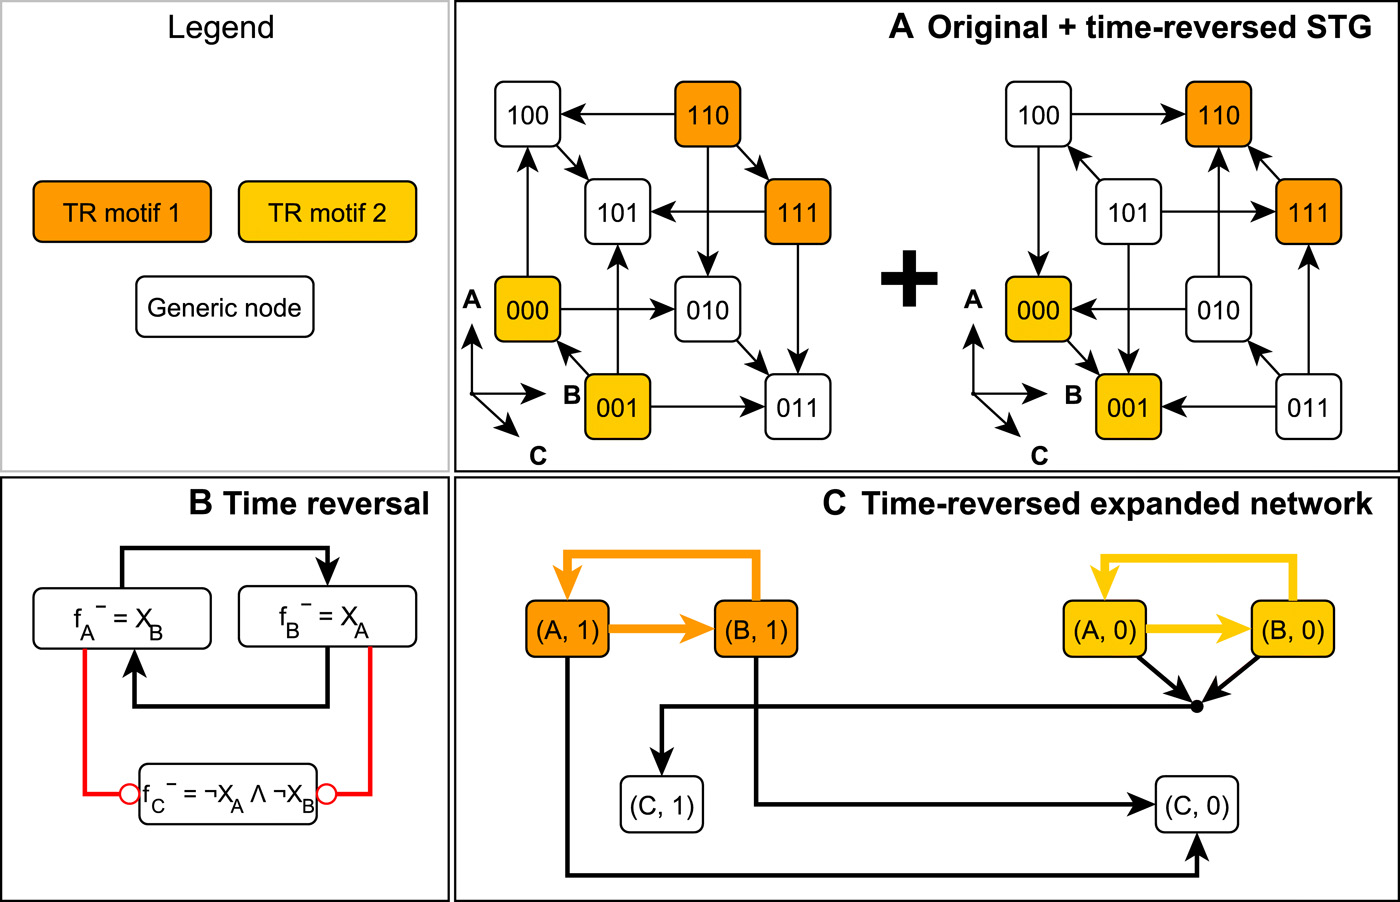
\includegraphics[scale=0.24]{Figures/time_reversal.jpeg}

\begin{tikzpicture}[remember picture, overlay]
  \only<2>{\node[below=-0.6cm of current page.west, blue, fill=green!10, xshift=6cm, text width=0.8\textwidth] (a-2) {- pystablemotifs builds the time-reversal BN and computes the maximal trap spaces of this BN by using PyBoolNet.\\- Of course, we can use Trappist to compute the maximal trap spaces of the time-reversal BN.};}
  
  \only<3>{\node[below=-1cm of current page.west, blue, fill=green!10, xshift=6cm, text width=0.8\textwidth] (a-3) {- Our \red{new finding} is that a maximal trap space of the time-reversal BN is equivalent to a \red{minimal conflict-free trap} of the Petri net encoding of the original BN.\\- We can easily adjust Trappist to compute minimal conflict traps with building \red{neither the time-reversal BN nor its Petri net encoding}.\\- In some cases, the Petri net building is quite \red{computationally intensive}~\cite{DBLP:conf/cmsb/TrinhBHS22}. It would be much helpful when we need to compute many terminal restriction spaces.};}
  
  \only<4>{\node[below=-1cm of current page.west, blue, fill=green!10, xshift=6cm, text width=0.8\textwidth] (a-4) {Jordan: The terminal restriction space is also computed based on LDOI (not only trap spaces of the time-reversal BN).\\Giang: I see. Let see the next slides.};}
\end{tikzpicture}

\end{frame}

\begin{frame}
\frametitle{Computation of terminal restriction spaces (cont.)}

\centering
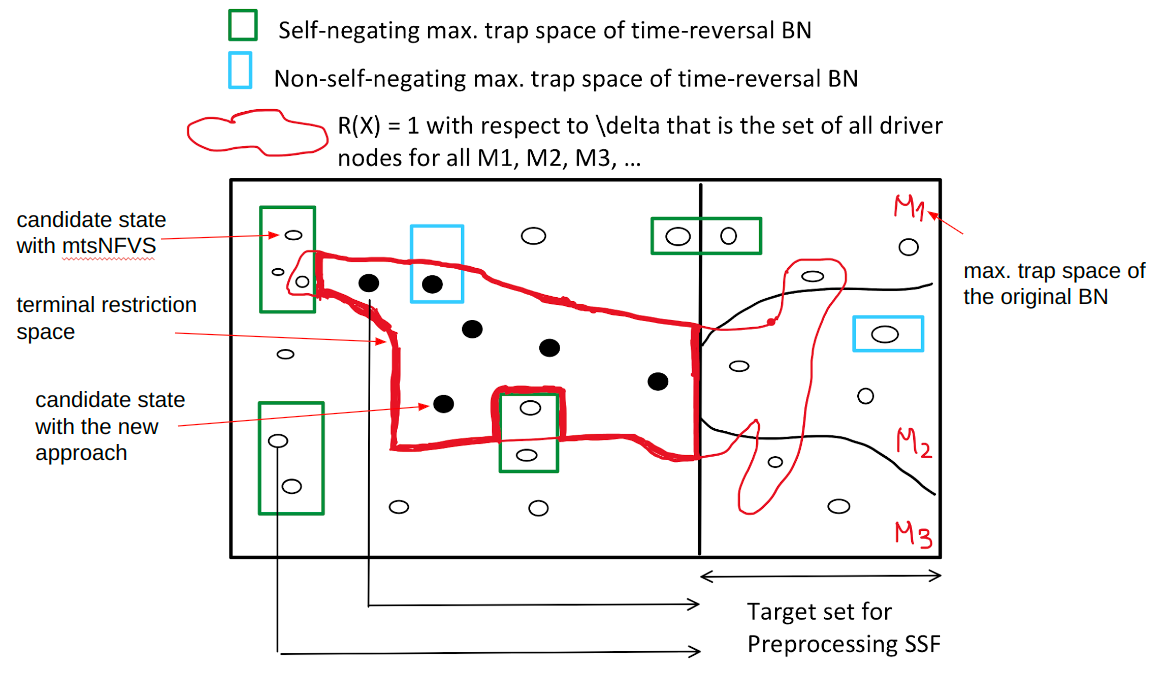
\includegraphics[scale=0.3]{Figures/terminal_restriction_space.png}

\begin{tikzpicture}[remember picture, overlay]
  \only<2>{\node[below=-3.5cm of current page.west, blue, fill=green!10, xshift=6cm, text width=0.8\textwidth] (a-2) {- I emphasize an \red{advantage} of the new approach.\\- The new candidate set seems to have shorter distances to the target set.\\- This is better for Preprocessing SSF as it may converge to the target set more quickly.};}
  
  \only<3>{\node[below=1.5cm of current page.west, blue, fill=green!10, xshift=6cm, text width=0.8\textwidth] (a-3) {- We can efficiently compute max. trap spaces of the time-reversal BN by using Trappist.\\- The self-negation of a max. trap space of the time-reversal BN can be checked by computing its LDOI in the original BN.};}
  
  \only<4>{\node[below=2cm of current page.west, blue, fill=green!10, xshift=6.6cm, text width=1\textwidth] (a-4) {- \(\Delta\) is the set of all virtual nodes that individually drive any stable motif.\\- A question is how to compute \(\Delta\) efficiently? Note that we need to compute \(\Delta\) \red{many times} in the whole process.\\- If the computation is \red{expensive}, we can ignore \(R(X)\). In this case, I hope that self-negating max. trap spaces are good enough.};}
  
  \only<5>{\node[below=2cm of current page.west, blue, fill=green!10, xshift=6.6cm, text width=1\textwidth] (a-5) {- The set of retained values \(B\) largely affects the size of the candidate set~\cite{GiangTCBB2020}.\\- One \red{interesting question} is that how we can propose heuristics for setting \(B\) based on the information about the terminal restriction space to get a smaller candidate set?};}
\end{tikzpicture}

\end{frame}

\begin{frame}
  \frametitle{Computation of candidate sets}

\centering
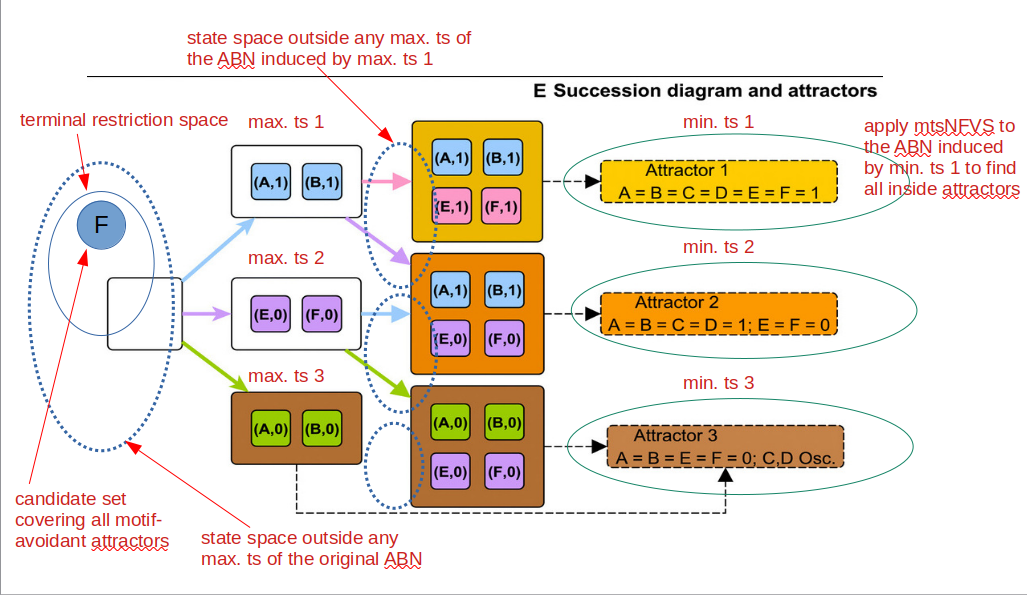
\includegraphics[scale=0.33]{Figures/general_approach.png}

\begin{tikzpicture}[remember picture, overlay]
  \only<1>{\node[below=-3.0cm of current page.center, blue, fill=green!10, xshift=2.2cm, text width=0.65\textwidth] (a-1) {- mtsNFVS uses PyBoolNet to compute the candidate set \(F\).\\- Again, we need replace PyBoolNet by a \red{more efficient} method for computing candidate sets.};}
  
  \only<2>{\node[below=-3.0cm of current page.center, blue, fill=green!10, xshift=2.2cm, text width=0.65\textwidth] (a-2) {- Since a fixed point is a special min. trap space, we can easily add more constraints to the ASP encoding of Trappist to make it able to compute \(F\).\\- In addition, we do not to build \red{a new BN} as mtsNFVS does~\cite{DBLP:conf/bcb/TrinhHB22}, everything can be performed in the Petri net encoding of the original BN.};}
\end{tikzpicture}

\end{frame}

\begin{frame}
\frametitle{Parallelization}

\centering
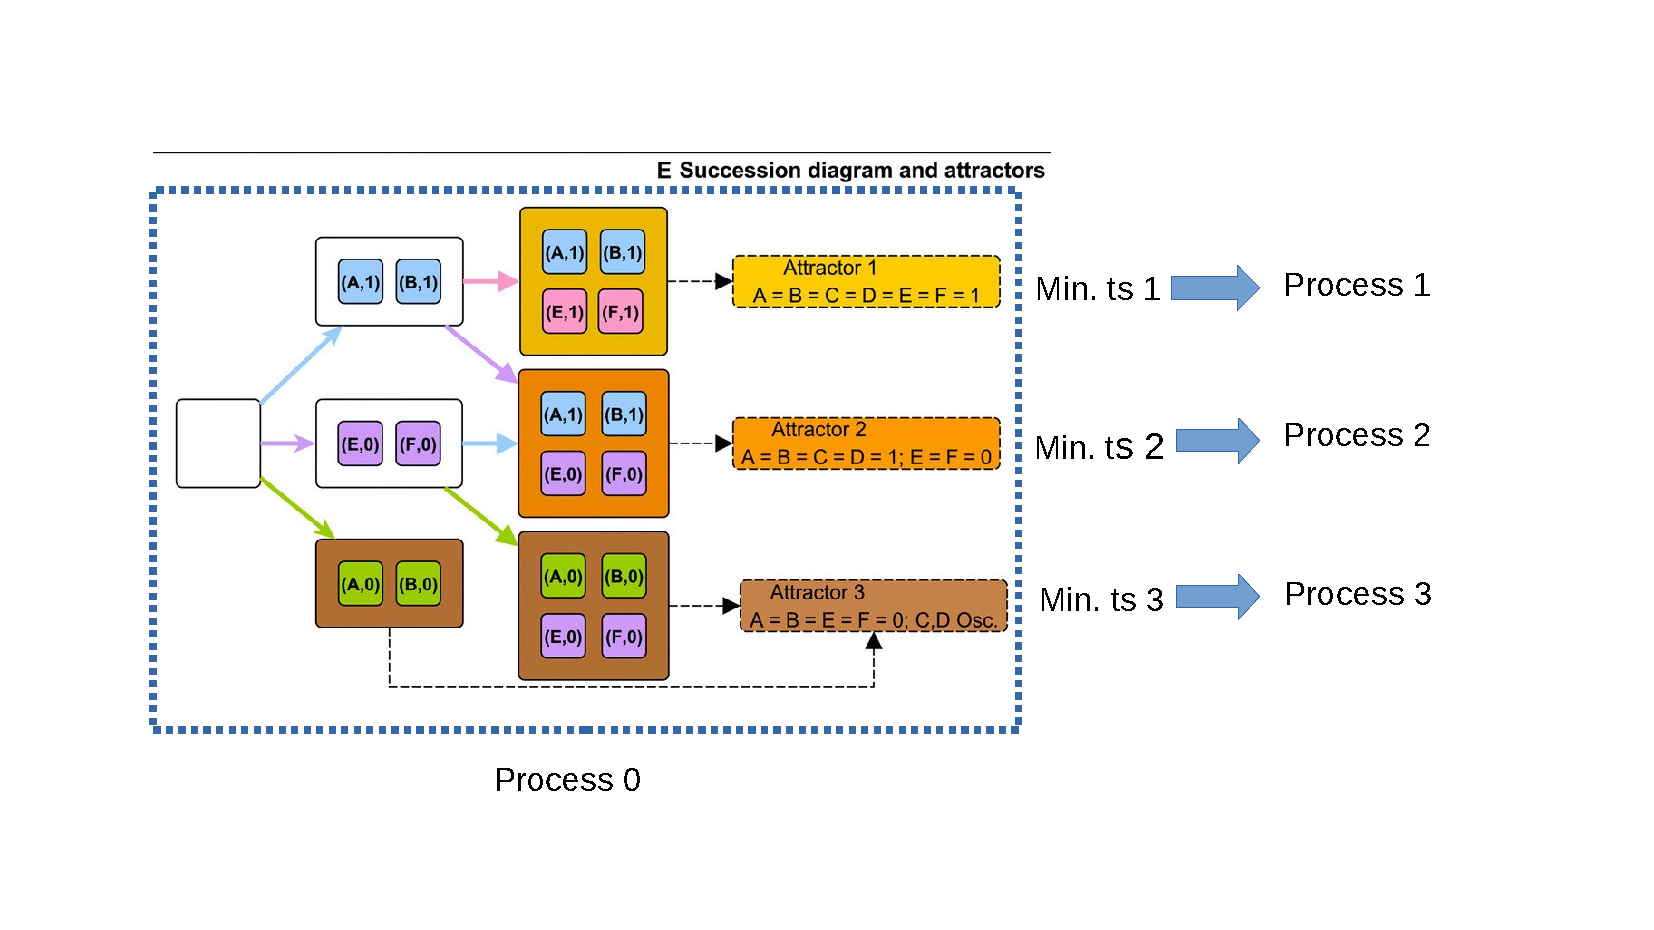
\includegraphics[scale=0.5]{Figures/Parallelization.pdf}

\begin{tikzpicture}[remember picture, overlay]
  \only<2>{\node[below=-1cm of current page.center, blue, fill=green!10, xshift=-2cm, text width=0.6\textwidth] (a-2) {- Process \(i\) is for computing concrete attractors inside minimal trap space \(i\). We can apply the approach of mtsNFVS to the reduced BN induced by \(i\).\\- Process 0 is for building the succession diagram and checking the existence of motif-avoidant attractors.};}
  
  \only<3>{\node[below=-1.5cm of current page.south, blue, fill=green!10, xshift=0cm, text width=0.8\textwidth] (a-3) {- Processes 0, 1, 2, ... can be completely paralleled.};}
  
  \only<4>{\node[below=-1.5cm of current page.south, blue, fill=green!10, xshift=0cm, text width=0.8\textwidth] (a-4) {- Process 0 can even be divided into many paralleled sub-processes.};}
\end{tikzpicture}

\end{frame}

\begin{frame}
  \frametitle{Target control}

After finishing the attractor detection phase, we will obtain the whole attractor landscape as well as the partial/full succession diagram.
If the succession diagram is full, its size should be \blue{moderate}.

\hspace{0.8cm}

The next step is how to compute \red{minimum control policies} that drive the network dynamics into a target attractor/min. trap space from any initial state?

\hspace{0.8cm}

There are some existing methods for the target control of asynchronous Boolean networks: CABEAN~\cite{DBLP:conf/fm/SuP21}, PyBoolNet~\cite{cifuentes2020control, cifuentes2021control}, pystablemotifs~\cite{Zaudo2015, rozum2021pystablemotifs}, AEON~\cite{Brim2021}.

\end{frame}

\begin{frame}[allowframebreaks]
  \frametitle{Target control: our observations}

CABEAN always ensures that the resulting control policies are minimum.
It relies on the calculation of strong basin of attraction, which may be very computationally expensive.

\hspace{0.8cm}

PyBoolNet exploits the information on trap spaces to find control policies.
However, it does not ensure that the resulting control policies are minimum.
It uses model checking to improve the quality of the control policies, which may be very computationally expensive as well.
Moreover, its scalability may be limited by the necessity to scan through the available perturbations.

\hspace{0.8cm}

pystablemotifs uses the succession diagram to find control policies.
However, it does not ensure that the resulting control policies are minimum.

\hspace{0.8cm}

AEON uses methods based on the computation of the strong basin, but with symbolic representation to exhaustively analyse all perturbations simultaneously. A postprocessing step is then needed to extract the minimal perturbations from the final result. Alternatively, if the network has parameters, such postprocessing can also be used to extract perturbations with favourable robustness within the parameter space. The method is mainly limited by the complexity of the symbolic state space search for all available perturbations.

\hspace{0.8cm}

In the reported experiments~\cite{DBLP:journals/bioinformatics/SuP21, DBLP:conf/fm/SuP21}, pystablemotifs is more time-efficient in most cases, though it did not return the minimum results in some cases.

\hspace{0.8cm}

In our opinion, pystablemotifs has much more potential than the others.
We should dive into it.
Of course, we need to improve both its \red{time-efficiency} and \red{accuracy}.

\end{frame}

\begin{frame}%[allowframebreaks]
\frametitle{Target control: more observations on PyBoolNet~\cite{cifuentes2020control}}

  \centering
  \begin{tikzpicture}[node distance = 2cm, auto]
    \node [draw, rectangle, fill=green!50, minimum height=2em] (target) {Phenotype};

    \node [draw, rectangle, fill=green!50, minimum height=2em, below=1.2cm of target] (BN) {Boolean network};
  
    \node [draw, rectangle, fill=green!50, minimum height=2em, right=1.2cm of BN] (i_trapspaces) {Intersected trap spaces};
  
    \node [draw, rectangle, fill=green!50, minimum height=2em, below=1.2cm of i_trapspaces] (PI) {Prime implicants};
  
    \node [draw, rectangle, fill=green!50, minimum height=2em, right=1.2cm of target] (s_trapspaces) {Selected trap spaces};
  
    \node [draw, rectangle, fill=green!50, minimum height=2em, right=1.2cm of s_trapspaces] (space_of_attraction) {Spaces of attraction};
  
    \node [draw, rectangle, fill=green!50, minimum height=2em, below=1.2cm of space_of_attraction] (control_strategies) {Control strategies};

    \draw [->] (target) -- (s_trapspaces);
    \draw [->] (target) -- (i_trapspaces);
    \draw [->] (BN) -- (PI);
    \draw [->] (PI) -- (i_trapspaces);
    \draw [->] (i_trapspaces) -- (s_trapspaces);
    \draw [->] (PI) -- (space_of_attraction);
    \draw [->] (s_trapspaces) -- (space_of_attraction);
    \draw [->] (space_of_attraction) -- (control_strategies);
    
    \only<2>{\node[above=0.2cm of i_trapspaces, red, text width=5cm, xshift=-2.5cm] (note-2) {compute\_trapspaces\_that\_intersect\_subspace};}

    \only<3>{\node[above=0.2cm of PI, red, text width=5cm, xshift=4cm] (note-3) {Used for percolation};}
  
    \only<4>{\node[above=0.2cm of space_of_attraction, red, text width=8cm, xshift=-3cm] (note-4) {Exploration of all possible sub-spaces whose numbers of fixed variables are up to \(\operatorname{min}(m, n)\) (\(m\) is the maximum size of the control strategies)};}
  
    \only<5>{\node[above=0.2cm of i_trapspaces, red, text width=8cm, xshift=0cm] (note-5) {The number of intersected trap spaces may be huge for large-scale models.};}
    \only<5>{\node[draw, rectangle, minimum height=3em, below=-1cm of i_trapspaces, red, text width=4.7cm] (e-5) {};}
  
    \only<6>{\node[below=0.5cm of PI, red, text width=8cm, xshift=0cm] (note-6) {The number of prime implicants may be huge for models with high average connectivity.};}
    \only<6>{\node[draw, rectangle, minimum height=3em, below=-1cm of PI, red, text width=4.7cm] (e-6) {};}
  
    \only<7>{\node[above=0.2cm of space_of_attraction, red, text width=7cm, xshift=-1.5cm] (note-7) {The number of explored sub-spaces is exponential in \(n\) in the worst case.};}
    \only<7>{\node[draw, rectangle, minimum height=3em, below=-1cm of space_of_attraction, red, text width=4cm] (e-7) {};}
  
  \end{tikzpicture}
\end{frame}

\begin{frame}%[allowframebreaks]
\frametitle{Target control: more observations on PyBoolNet~\cite{FontanalsLaura2022}}

  \centering
  \begin{tikzpicture}[node distance = 2cm, auto]
    \node [draw, rectangle, fill=green!50, minimum height=2em] (target) {Phenotype};

    \node [draw, rectangle, fill=green!50, minimum height=2em, below=1.2cm of target] (BN) {Boolean network};
  
    \node [draw, rectangle, fill=green!50, minimum height=2em, right=1.2cm of BN] (i_trapspaces) {Intersected trap spaces};
  
    \node [draw, rectangle, fill=green!50, minimum height=2em, below=1.2cm of i_trapspaces] (PI) {Prime implicants};
  
    \node [draw, rectangle, fill=green!50, minimum height=2em, right=1.2cm of target] (s_trapspaces) {Selected trap spaces};
  
    \node [draw, rectangle, fill=green!50, minimum height=2em, right=1.2cm of s_trapspaces] (space_of_attraction) {Spaces of attraction};
  
    \node [draw, rectangle, fill=green!50, minimum height=2em, below=1.2cm of space_of_attraction] (control_strategies) {Control strategies};

    \draw [->] (target) -- (s_trapspaces);
    \draw [->] (target) -- (i_trapspaces);
    \draw [->] (BN) -- (PI);
    \draw [->] (PI) -- (i_trapspaces);
    \draw [->] (i_trapspaces) -- (s_trapspaces);
    \draw [->] (PI) -- (space_of_attraction);
    \draw [->] (s_trapspaces) -- (space_of_attraction);
    \draw [->] (space_of_attraction) -- (control_strategies);
  
    \only<1>{\node[above=0.2cm of space_of_attraction, red, text width=7cm, xshift=-1.5cm] (note-1) {The number of explored sub-spaces is exponential in \(n\) in the worst case.};}
    \only<1->{\node[draw, rectangle, minimum height=3em, below=-1cm of space_of_attraction, red, text width=4cm] (e-1-1) {};}
    
    \only<1->{\node[draw, rectangle, minimum height=3em, below=-1cm of i_trapspaces, red, text width=4.7cm] (e-1-2) {};}
  
    \only<1->{\node[draw, rectangle, minimum height=3em, below=-1cm of PI, red, text width=4.7cm] (e-1-3) {};}
    
    \only<2>{\node[above=0.2cm of space_of_attraction, red, text width=7cm, xshift=-1.5cm] (note-2) {Propose a new implementation for this step based on ASP.};}
    
    \only<3>{\node[above=0.2cm of space_of_attraction, red, text width=6cm, xshift=-1.5cm] (note-2) {It is possible to optimize the ASP encoding.};}
  
    \only<4>{\node[above=0.2cm of space_of_attraction, red, text width=11cm, xshift=-3.5cm] (note-2) {However, even with an optimal ASP encoding, the running time of the ASP solver may still large because the search space of the problem itself is intrinsically huge (\(\mathcal{O}(\sum_{k = 1}^{\operatorname{min}(m, n)}2^i \times \binom{n}{k})\)).};}
    
    \only<5>{\node[above=0.2cm of space_of_attraction, red, text width=6cm, xshift=-1.5cm] (note-2) {Hence, we retain the opinion that pystablemotifs has much more potential than the others.};}
  \end{tikzpicture}
\end{frame}

\begin{frame}%[allowframebreaks]
\frametitle{Some potential improvements to PyBoolNet~\cite{FontanalsLaura2022}}

  \centering
  \begin{tikzpicture}[node distance = 2cm, auto]
    \node [draw, rectangle, fill=green!50, minimum height=2em] (target) {Phenotype};

    \node [draw, rectangle, fill=green!50, minimum height=2em, below=1.2cm of target] (BN) {Boolean network};
  
    \node [draw, rectangle, fill=green!50, minimum height=2em, right=1.2cm of BN] (i_trapspaces) {Intersected trap spaces};
  
    \node [draw, rectangle, fill=green!50, minimum height=2em, below=1.2cm of i_trapspaces] (PI) {Prime implicants};
  
    \node [draw, rectangle, fill=green!50, minimum height=2em, right=1.2cm of target] (s_trapspaces) {Selected trap spaces};
  
    \node [draw, rectangle, fill=green!50, minimum height=2em, right=1.2cm of s_trapspaces] (space_of_attraction) {Spaces of attraction};
  
    \node [draw, rectangle, fill=green!50, minimum height=2em, below=1.2cm of space_of_attraction] (control_strategies) {Control strategies};

    \draw [->] (target) -- (s_trapspaces);
    \draw [->] (target) -- (i_trapspaces);
    \draw [->] (BN) -- (PI);
    \draw [->] (PI) -- (i_trapspaces);
    \draw [->] (i_trapspaces) -- (s_trapspaces);
    \draw [->] (PI) -- (space_of_attraction);
    \draw [->] (s_trapspaces) -- (space_of_attraction);
    \draw [->] (space_of_attraction) -- (control_strategies);
  
    \only<1>{\node[draw, rectangle, minimum height=3em, below=-1cm of PI, red, text width=4.7cm] (e-1-1) {};}
    
    \only<1>{\node[draw, rectangle, minimum height=3em, below=-1cm of i_trapspaces, red, text width=4.7cm] (e-1-2) {};}
  
    \only<1>{\node[draw, rectangle, minimum height=3em, below=-1cm of space_of_attraction, red, text width=4cm] (e-1-3) {};}
    
    \only<2>{\node[below=0.5cm of PI, red, text width=8cm, xshift=0cm] (note-2-1) {Use Trappist.};}
    \only<2>{\node[draw, rectangle, minimum height=9em, below=-1.3cm of i_trapspaces, red, text width=4cm] (e-2-1) {};}
    \only<2>{\node[draw, rectangle, minimum height=3em, below=-1cm of target, red, text width=3cm] (e-2-2) {};}
    \only<2>{\node[below=0.2cm of target, red, text width=6cm, xshift=2cm] (note-2-2) {Target can be a minimal trap space.};}
    
    \only<3>{\node[draw, rectangle, minimum height=3em, below=-1cm of space_of_attraction, red, text width=4cm] (e-3) {};}
    \only<3>{\node[above=0.2cm of space_of_attraction, red, text width=8cm, xshift=-2.5cm] (note-3) {However, we need to adjust the ASP encoding because it relies on prime implicants. The new ASP encoding should rely on Boolean functions instead.};}
    
    \only<4>{\node[below=0.5cm of PI, red, text width=8cm, xshift=0cm] (note-4) {The bottleneck on the number of intersected trap spaces still remains.};}
    \only<4>{\node[draw, rectangle, minimum height=9em, below=-1.3cm of i_trapspaces, red, text width=4cm] (e-4) {};}
    
    \only<5>{\node[below=0.5cm of PI, red, text width=8cm, xshift=0cm] (note-5) {We can use BDDs to compute and represent the set of intersected trap spaces (also the set of selected trap spaces).};}
    \only<5>{\node[draw, rectangle, minimum height=13.2em, below=-2.9cm of i_trapspaces, red, text width=4.7cm, xshift=-0.3cm] (e-5) {};}
    
    \only<6>{\node[draw, rectangle, minimum height=3em, below=-1cm of space_of_attraction, red, text width=4cm] (e-6) {};}
    \only<6>{\node[above=0.2cm of space_of_attraction, red, text width=8cm, xshift=-2.5cm] (note-6) {However, we need to adjust the ASP encoding because it relies on the set of selected trap spaces. We need to encode the BDD as ASP rules.};}
    
    \only<7>{\node[draw, rectangle, minimum height=3em, below=-1cm of space_of_attraction, red, text width=4cm] (e-7) {};}
    \only<7>{\node[above=0.2cm of space_of_attraction, red, text width=11cm, xshift=-3.5cm] (note-7) {Along with optimizing the ASP encoding, I wonder if we can write a conference paper based on these new ideas. Of course, the first thing we need to do is to develop a concrete method, implement it, and then test it on large real-world models.};}
    
  \end{tikzpicture}
\end{frame}

\begin{frame}
\frametitle{Target control with the full succession diagram}

\centering
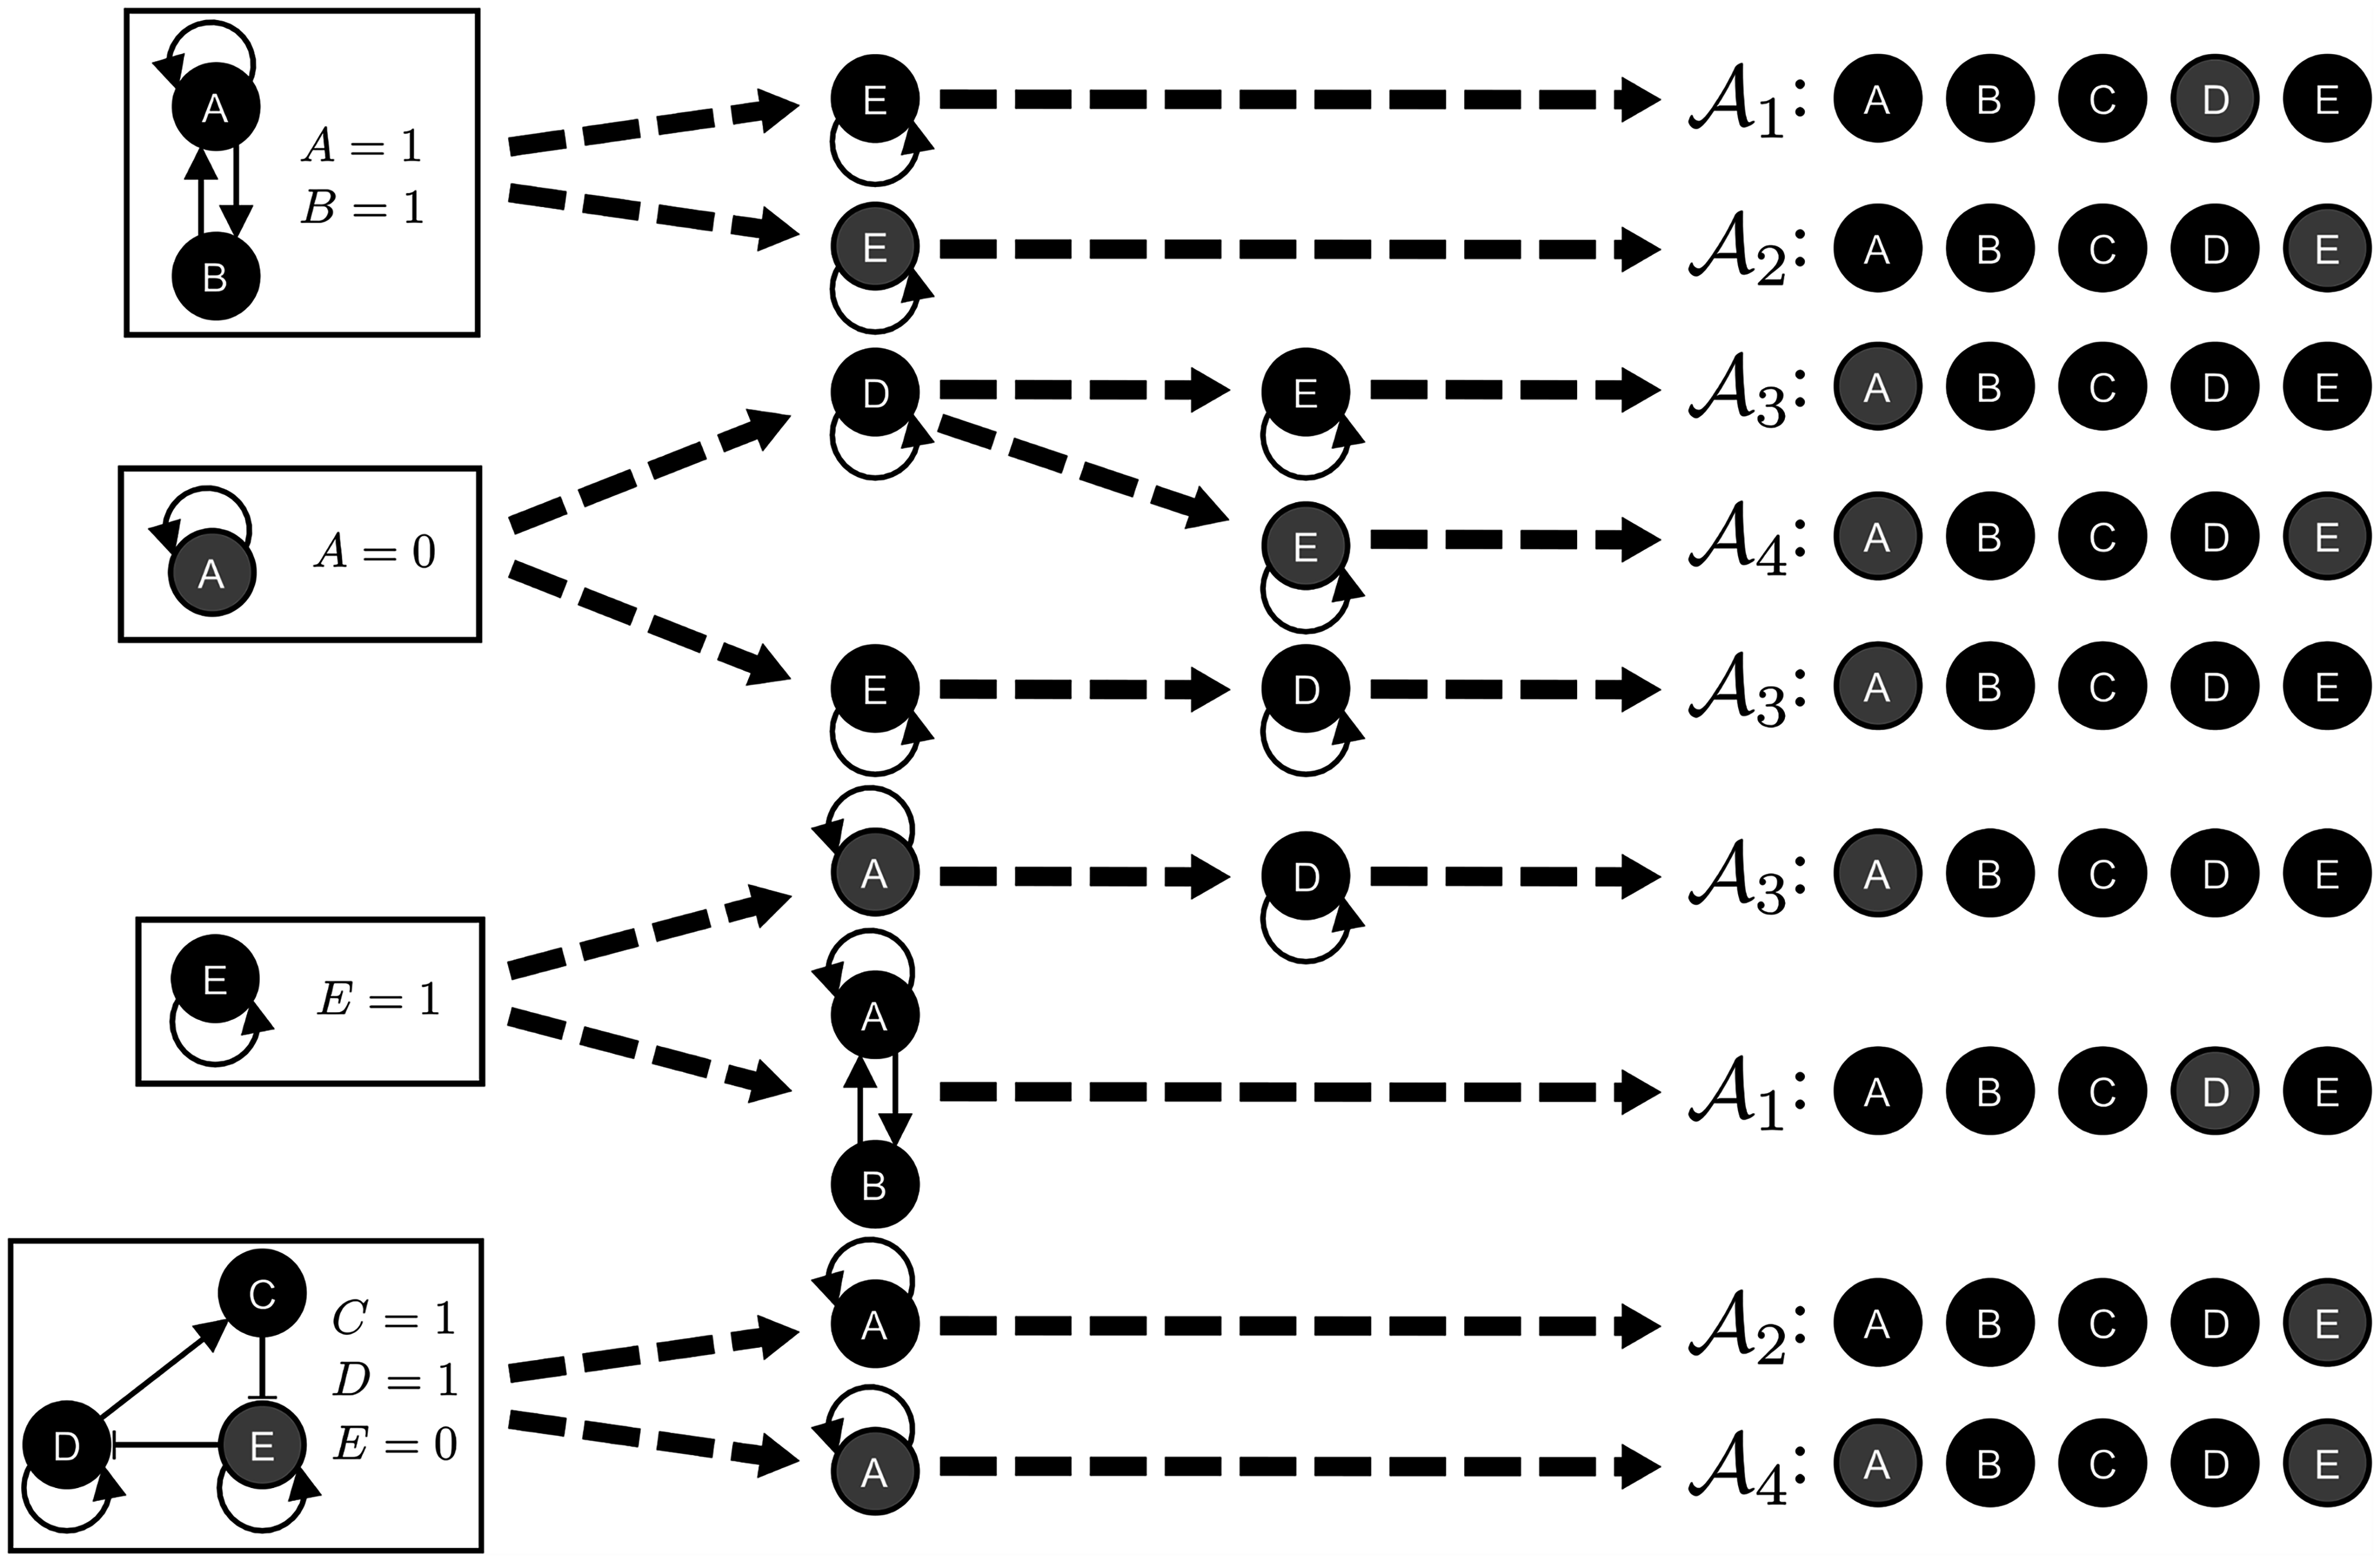
\includegraphics[scale=0.6]{Figures/target_control_full.png}

\begin{tikzpicture}[remember picture, overlay]
  \only<2>{\node[below=-1cm of current page.center, blue, fill=green!10, xshift=-2cm, text width=0.6\textwidth] (a-2) {- In this case, we simply reuse the approach of pystablemotifs.\\- Specifically, we follow all the paths in the full succession diagram leading to the target attractor to find driver nodes.};}
\end{tikzpicture}

\end{frame}

\begin{frame}
\frametitle{Target control with the partial succession diagram}

\centering
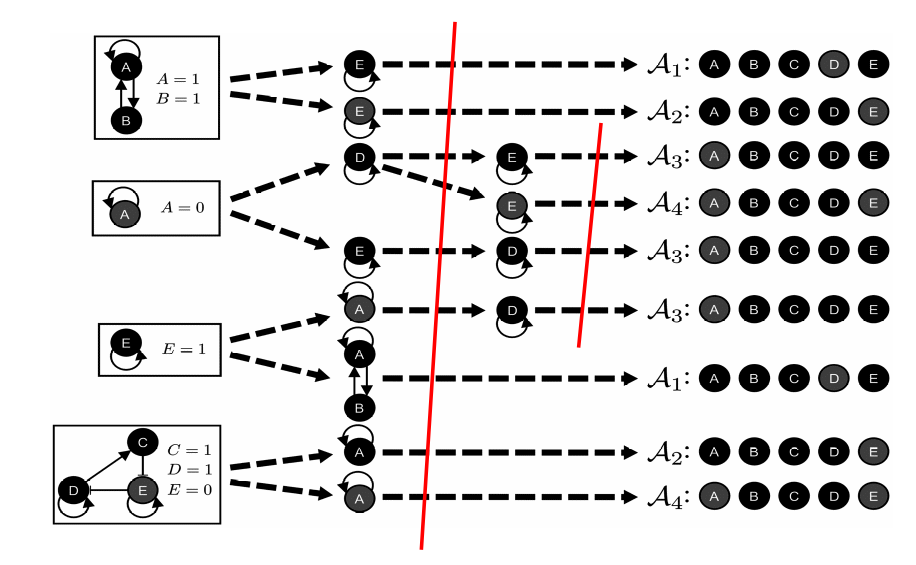
\includegraphics[scale=0.35]{Figures/target_control_partial.png}

\begin{tikzpicture}[remember picture, overlay]
  \only<2>{\node[below=-1cm of current page.center, blue, fill=green!10, xshift=-2cm, text width=0.6\textwidth] (a-2) {- In this case, we need only to rebuild the new succession diagram \red{induced} by the target attractor (i.e., it only contains the paths in the full succession diagram leading to the target attractor).\\- Note that in the rebuilding, we do not need to compute the stable motifs \red{already computed} in the attractor detection phase.};}
  
  \only<3>{\node[below=2cm of current page.center, blue, fill=green!10, xshift=-2cm, text width=0.6\textwidth] (a-3) {- For example, consider the target attractor as \(\mathcal{A}_3\). The induced succession diagram includes only three paths.};}
  
  \only<3>{\node[below=1cm of current page.center, blue, fill=green!10, xshift=-2cm, text width=0.6\textwidth] (a-4) {- One question may be whether we need to compute both \(\{E = 1\}\) and \(\{E = 0\}\). No, we \red{do not need}. We have already known the target attractor, hence we can add constraints to the ASP encoding to guide Trappist for searching only stable motifs that are \red{compatible} with the target attractor \(\mathcal{A}_3\).};}
  
  \only<4>{\node[below=1cm of current page.center, blue, fill=green!10, xshift=-1cm, text width=0.6\textwidth] (a-4) {- Finally, we follow the \red{induced} succession diagram to find driver nodes (similar to the case of the full succession diagram).\\- The induced succession diagram may be \red{much smaller} than the full one, hence the computational burden may be reduced significantly.};}
  
  \only<5>{\node[below=0cm of current page.center, blue, fill=green!10, xshift=-1cm, text width=0.8\textwidth] (a-5) {Jordan: The control approach of pystablemotifs is independent to the update scheme. CABEAN is designed for asynchronous Boolean networks. Hence, the problem of not obtaining the minimum control polices is not really mattered with pystablemotifs.\\Giang: I understand. Let me recall the control example.};}
\end{tikzpicture}

\end{frame}

\begin{frame}
\frametitle{Control features}

\begin{center}
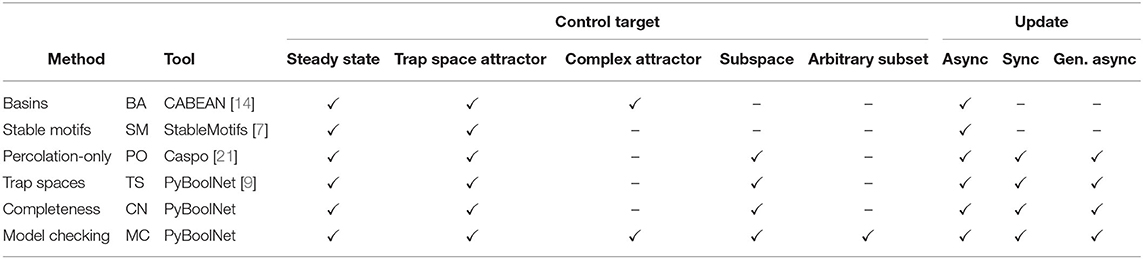
\includegraphics[scale=0.3]{Figures/control_approach.jpg}
\end{center}

\only<1>{Model checking-based method~\cite{CifuentesFontanals2022}\footnote{Cifuentes-Fontanals L, Tonello E and Siebert H (2022) Control in Boolean Networks With Model Checking. Front. Appl. Math. Stat. 8:838546. doi: 10.3389/fams.2022.838546}}

\only<2>{I hope to develop more \blue{control features} for nfvs-motifs: complex attractor, sub-space, arbitrary subset. I am thinking about this.}

\end{frame}

\begin{frame}
\frametitle{Model checking-based method~\cite{CifuentesFontanals2022}}

\begin{center}
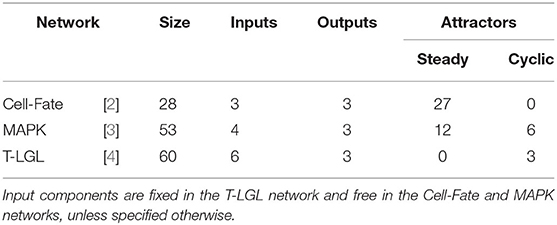
\includegraphics[scale=0.4]{Figures/MC_data_set.jpg}
\end{center}

\only<1>{The running time of the model checking-based method (MC) is large (\red{several hours}).}

\only<2>{We can see that MC seems \red{to be not time-efficient} for large-scale models.}

\only<3>{It would be great if nfvs-motifs can provide all features as MC does but run much rapidly.}

\end{frame}


\begin{frame}
  \frametitle{Improve the accuracy}

Consider the example asynchronous Boolean network (Figure 2 in~\cite{cifuentes2021control}).
\begin{columns}
  \begin{column}{0.4\textwidth}
    \begin{equation*}
      \begin{cases}
        f_1 = \neg x_2 \lor (x_1 \land \neg x_3)\\
        f_2 = (x_1 \land \neg x_3) \lor (x_2 \land x_3)\\
        f_3 = (\neg x_1 \land \neg x_2) \lor (x_2 \land x_3)\\
      \end{cases}
    \end{equation*}
  \end{column}
  \begin{column}{0.6\textwidth}
    \centering
    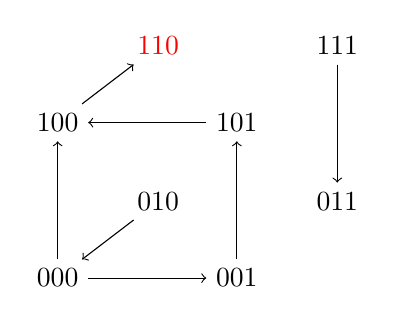
\begin{tikzpicture}[node distance=0.5cm and 0.5cm, every node/.style={scale=1.0}]
   \node[] (0) [] {000};
   \node[] (1) [right=of 0, xshift=1cm] {001};
   \node[] (2) [above right=of 0] {010};
   \node[] (3) [right=of 2, xshift=1cm] {011};
   \node[] (4) [above=of 0, yshift=1cm] {100};
   \node[] (5) [right=of 4, xshift=1cm] {101};
   \node[red] (6) [above=of 2, yshift=1cm] {110};
   \node[] (7) [above=of 3, yshift=1cm] {111};

  \draw[->] (0) edge [] (1);
  \draw[->] (0) edge [] (4);
    \draw[->] (1) edge [] (5);
    \draw[->] (2) edge [] (0);
    \draw[->] (4) edge [] (6);
    \draw[->] (5) edge [] (4);
    \draw[->] (7) edge [] (3);
   
    \end{tikzpicture}
  \end{column}
\end{columns}

\hspace{0.8cm}

The result of pystablemotifs is \red{\(\{x_1 = 1, x_3 = 0\}\)}.
The result of CABEAN (also of PyBoolNet with model checking) is \blue{\(\{x_3 = 0\}\)}.

\hspace{0.8cm}

We have obtained a \blue{preliminary idea} for improving the accuracy of pystablemotifs.
However, we need to make it more specific as well as investigate its efficiency.
In most cases, smaller control policies, longer computational time.
We will present it in the next slides.

\end{frame}

\begin{frame}
  \frametitle{Improve the accuracy (cont.)}

\only<1>{Consider the \red{synchronous} counterpart of the previous asynchronous Boolean network.}

\only<-2>{
\begin{columns}
  \begin{column}{0.4\textwidth}
    \begin{equation*}
      \begin{cases}
        f_1 = \neg x_2 \lor (x_1 \land \neg x_3)\\
        f_2 = (x_1 \land \neg x_3) \lor (x_2 \land x_3)\\
        f_3 = (\neg x_1 \land \neg x_2) \lor (x_2 \land x_3)\\
      \end{cases}
    \end{equation*}
  \end{column}
  \begin{column}{0.6\textwidth}
    \centering
    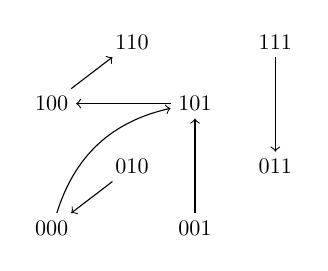
\begin{tikzpicture}[node distance=0.4cm and 0.4cm, every node/.style={scale=0.8}]
      \node[] (0) [] {000};
      \node[] (1) [right=of 0, xshift=1cm] {001};
      \node[] (2) [above right=of 0] {010};
      \node[] (3) [right=of 2, xshift=1cm] {011};
      \node[] (4) [above=of 0, yshift=1cm] {100};
      \node[] (5) [right=of 4, xshift=1cm] {101};
      \node[] (6) [above=of 2, yshift=1cm] {110};
      \node[] (7) [above=of 3, yshift=1cm] {111};

      \draw[->] (0) edge [bend left] (5);
      \draw[->] (1) edge [] (5);
      \draw[->] (2) edge [] (0);
      \draw[->] (4) edge [] (6);
      \draw[->] (5) edge [] (4);
      \draw[->] (7) edge [] (3);
    \end{tikzpicture}
  \end{column}
\end{columns}
}

\hspace{0.5cm}

\only<2>{Assume that the target attractor is \red{\(\{110\}\)}.
The result of pystablemotifs is \red{\(\{x_1 = 1, x_3 = 0\}\)}.
The minimum result still should be \blue{\(\{x_3 = 0\}\)}.}

\hspace{0.5cm}

\only<3->{
\begin{columns}
  \begin{column}{0.4\textwidth}
    \begin{equation*}
      \begin{cases}
        f_1 = \neg x_2 \lor x_1\\
        f_2 = x_1\\
      \end{cases}
    \end{equation*}
  \end{column}
  \begin{column}{0.6\textwidth}
    \centering
    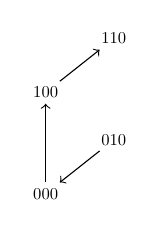
\begin{tikzpicture}[node distance=0.4cm and 0.4cm, every node/.style={scale=0.6}]
      \node[] (0) [] {000};
      \node[] (2) [above right=of 0] {010};
      \node[] (4) [above=of 0, yshift=1cm] {100};
      \node[] (6) [above=of 2, yshift=1cm] {110};

      \draw[->] (0) edge [] (4);
      \draw[->] (2) edge [] (0);
      \draw[->] (4) edge [] (6);
    \end{tikzpicture}
  \end{column}
\end{columns}
}

\only<3>{\(\{x_1 = 1, x_3 = 0\}\) is a stable motif obtained by pystablemotifs.
The function \texttt{minimal\_drivers} (in the file \texttt{drivers.py}) finds the minimum subsets of stable motif’s states that, when fixed in the logical model, are enough to force the state of every node in the motif into the stable motif \(M\).
This function considers all subsets of size 1, 2, ..., \(|M| - 1\) and relies on LDOI (\texttt{implied,contradicted = logical\_domain\_of\_influence(driver\_dict,primes)}).}

\hspace{0cm}

\only<3>{In the example, \(\{x_3 = 0\}\) cannot be obtained by using this method.}

\only<4>{I guess if we use DOI instead of LDOI, we can get \(\{x_3 = 0\}\) instead of \(\{x_1 = 1, x_3 = 0\}\). However, calculating DOI can be \red{difficult} in general.}

\hspace{0.5cm}

\only<4>{\textbf{Research question}: How to develop \blue{an efficient algorithm} for driver node identification in a stable motif regardless of update schemes?}

\hspace{0.5cm}

\only<4>{The \blue{efficient} word means that the algorithm is \blue{fast} and can return \blue{smaller} (maybe not optimal) sets of drive nodes.}

\end{frame}

\begin{frame}
  \frametitle{Ideas for driver node identification}

\only<1>{
From the previous example, we observed that:
\begin{itemize}
  \item If fixing \(x_1 = 1\), the resulting BN has two max. trap spaces \(\{x_3 = 0\}\) and \red{\(\{x_2 = 1, x_3 = 1\}\)}. The latter is not compatible with the stable motif \(\{x_1 = 1, x_3 = 0\}\).
  \item If fixing \(x_3 = 0\), the resulting BN has only one max. trap space \(\{x_1 = 1\}\). All max. trap spaces are compatible with the stable motif \(\{x_1 = 1, x_3 = 0\}\).
\end{itemize}

\hspace{0.5cm}
}

\only<1>{
We formulate a problem as follows.

\begin{block}{Driver node identification}
Let \(\mathcal{N}\) be a BN and \(M = \{x_{i_1} = a_{i_1}, ..., x_{i_k} = a_{i_k}\}\) be a max. trap space of \(\mathcal{N}\). Find all minimum subsets \(S\) of \(M\) such that of max. trap spaces of the new BN induced by \(S\) are compatible with \(M\). 
\end{block}

This problem is related to \red{the fixed point control problem} considered in~\cite{Biane2019, Moon2022}.

\hspace{0.5cm}
}

\only<2>{
We can solve this problem by using \blue{answer set programming}. The main idea is as follows.

\begin{itemize}
  \item Consider the nodes in \(M\) as controllable nodes (\red{\(x_1, x_3\)}) and the remaining nodes as uncontrollable nodes (\red{\(x_2\)}).
  \item Introduce an auxiliary Boolean variable \(d_i\) for each controllable node \(x_i\) (\red{\(d_1, d_3\)}). If \(d_i = 1\), node \(x_i\) is fixed to \(a_i\). If \(d_i = 0\), node \(x_i\) is updated by using its original Boolean function. 
  \item Let \(\mathcal{L}\) be the ASP characterizing the trap spaces of \(\mathcal{N}\) considering all \(d_i\). Let \(C\) be the constraint characterizing the max. trap space \(M\) (\red{\(x_1 = 1 \land x_3 = 0\)}).
  \item Compute the set \(A\) of minimal answer sets (projecting only \(d_i\) not \(x_i\)) of \(\mathcal{L}\) + \(C\). \red{\(A = \{\{d_1\}, \{d_3\}\}\)}
  \item Compute the set \(A'\) of minimal answer sets (projecting only \(d_i\) not \(x_i\)) of \(\mathcal{L}\) + \(\neg C\) + \(A\). \red{\(A' = \{\{d_1\}\}\)}
  \item Return \(A \setminus A'\). \red{Return \(\{\{d_3\}\}\)} where \(\{d_3\}\) corresponds to \(\{x_3 = 0\}\)
\end{itemize}

\hspace{0.5cm}
}

\only<3>{
This ASP-based method can avoid considering explicitly all subsets of size 1, 2, ..., \(|M| - 1\). This exploits the power of ASP solvers (e.g., clingo).

\hspace{0.5cm}

However, it is still needed to test its efficiency in practice.
Moreover, we also need to investigate its correctness thoroughly.
}

\end{frame}

\begin{frame}
  \frametitle{Bottlenecks of both pystablemotifs and mtsNFVS}

\only<1>{
The new approach still encounters the two \red{bottlenecks} of both pystablemotifs and mtsNFVS.

\hspace{0.1cm}
}

\only<2>{
The case of many source nodes where there are actually too many attractors (at least \(2^k\) where \(k\) is the number of source nodes).
mtsNFVS is less affected than pystablemotifs, but this is still problem because mtsNFVS uses the set of \red{explicit} (not \blue{symbolic}) min. trap spaces.

\hspace{0.1cm}

We have found a wise way to symbolically represent the \blue{maximal answer sets} (corresponding to \blue{min. trap spaces}) of the encoded ASP characterizing all trap spaces.

\hspace{0.1cm}

For \red{max. trap spaces}, we need to adjust the current method. We are thinking about this.
}

\only<3>{
There exist some very huge attractors inside min. trap spaces.
In this case, the number free variables of a min. trap space is \red{still too large} (even all the nodes of the original network).
pystablemotifs only ends with min. trap spaces.
It is \red{very hard} for mtsNFVS to reach the best case (i.e., \(|F| = 1\)) to avoid the reachability analysis.

\hspace{0.1cm}

\sout{One example is the model shown in~\url{https://github.com/jcrozum/pystablemotifs/issues/83}.
This network has no stable motifs, and we have exactly one attractor for each combination of source node values.}

\hspace{0.1cm}

Our general idea is as follows.

\begin{itemize}
  \item We have the \blue{information} about the min. trap space. We can use this information to guide Preprocessing SSF to reach the easy cases where we can avoid or at least reduce the reachability analysis times.
\end{itemize}
}

\end{frame}

\begin{frame}
\frametitle{Deal with the issue of huge attractors}

This is a very rare case.
We can anticipate it in advance via the information about the number of free nodes of the min. trap space.

\hspace{0.1cm}

In this case, it is \red{harder} for Preprocessing SSF to converge into \blue{one state} (i.e., the best case where we do not need to check the reachability).

\hspace{0.1cm}

However, we know that it is \blue{likely} that there is only one huge attractor and all candidate states are in this attractor.

\end{frame}

\begin{frame}
\frametitle{Deal with the issue of huge attractors (cont.)}

My idea is as follows.
\begin{itemize}
  \item First, choose a pivot state \(s^{p}\) from the candidate set \(F_m\).
  \item Second, from \(s^{p}\) create and gradually enlarge a "trap" to attract other states in \(F_m\). The trap is the set of states that can be reach \(s^{p}\).
  \item Third, perform Preprocessing SSF and the enlargement in parallel. When a state converges into the trap, we can exclude it from \(F_m\).
  \item Finally, we have \(F_m\) with the expectation that it contains only the pivot state.
\end{itemize}

\hspace{0.1cm}

The principle is that \blue{larger trap}, \blue{more possibility} to converge it.

\end{frame}

\begin{frame}
\frametitle{Deal with the issue of huge attractors (cont.)}

\begin{columns}
  \begin{column}{0.4\textwidth}
    \centering
    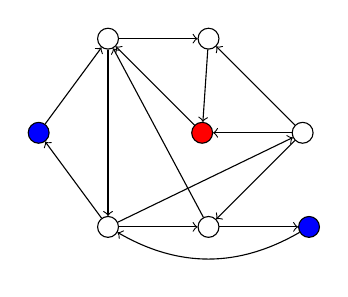
\begin{tikzpicture}[node distance=1cm and 1cm, every node/.style={scale=0.8}]
      \node[circle, draw, fill=red] (1) [] {};
      \node[circle, draw] (4) [right=of 1] {};
      \node[circle, draw] (2) [above left=of 1, yshift=0cm] {};
      \node[circle, draw] (3) [right=of 2] {};
      
      \node[circle, draw, fill=blue] (7) [left=of 1, xshift=-1cm] {};
      \node[circle, draw] (5) [below left=of 4, yshift=0cm] {};
      \node[circle, draw, fill=blue] (8) [right=of 5, yshift=0cm] {};
      \node[circle, draw] (6) [left=of 5, yshift=0cm] {};

      \draw[->] (1) edge [] (2);
      \draw[->] (2) edge [] (3);
      \draw[->] (2) edge [] (6);
      \draw[->] (3) edge [] (1);
      \draw[->] (4) edge [] (1);
      \draw[->] (4) edge [] (3);
      \draw[->] (4) edge [] (5);
      \draw[->] (5) edge [] (2);
      \draw[->] (5) edge [] (8);
      \draw[->] (6) edge [] (4);
      \draw[->] (6) edge [] (5);
      \draw[->] (6) edge [] (7);
      \draw[->] (7) edge [] (2);
      \draw[->] (8) edge [bend left] (6);
    \end{tikzpicture}
  \end{column}
  \begin{column}{0.6\textwidth}
    \centering
    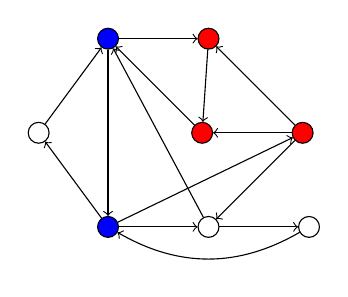
\begin{tikzpicture}[node distance=1cm and 1cm, every node/.style={scale=0.8}]
      \node[circle, draw, fill=red] (1) [] {};
      \node[circle, draw, fill=red] (4) [right=of 1] {};
      \node[circle, draw, fill=blue] (2) [above left=of 1, yshift=0cm] {};
      \node[circle, draw, fill=red] (3) [right=of 2] {};
      
      \node[circle, draw] (7) [left=of 1, xshift=-1cm] {};
      \node[circle, draw] (5) [below left=of 4, yshift=0cm] {};
      \node[circle, draw] (8) [right=of 5, yshift=0cm] {};
      \node[circle, draw, fill=blue] (6) [left=of 5, yshift=0cm] {};

      \draw[->] (1) edge [] (2);
      \draw[->] (2) edge [] (3);
      \draw[->] (2) edge [] (6);
      \draw[->] (3) edge [] (1);
      \draw[->] (4) edge [] (1);
      \draw[->] (4) edge [] (3);
      \draw[->] (4) edge [] (5);
      \draw[->] (5) edge [] (2);
      \draw[->] (5) edge [] (8);
      \draw[->] (6) edge [] (4);
      \draw[->] (6) edge [] (5);
      \draw[->] (6) edge [] (7);
      \draw[->] (7) edge [] (2);
      \draw[->] (8) edge [bend left] (6);
    \end{tikzpicture}
  \end{column}
\end{columns}

\hspace{0.8cm}

How to efficiently enlarge the trap (i.e., computing predecessors)?
Using BDDs as in~\cite{DBLP:journals/bioinformatics/GargCXMM08, DBLP:conf/cav/BenesBPS21}?

\hspace{0.8cm}

Thanks to \blue{time-reversal}, we can compute successors (instead of predecessors in the original ABN) in the time-reversal ABN.

\hspace{0.8cm}

This process can purely rely on the function evaluation (not BDDs or unfoldings).
Hence, it is expected to be viable for very large models.
\end{frame}

\begin{frame}
\frametitle{Deal with the issue of huge attractors (cont.)}

\footnotesize
\begin{columns}
  \begin{column}{0.4\textwidth}
    \begin{equation*}
      \begin{cases}
        v_1, \neg v_1 \land v_2 \land \neg v_3\\
        v_2, \neg v_1 \lor \neg v_3\\
        v_3, \neg v_1 \land v_2 \land \neg v_3\\
      \end{cases}
    \end{equation*}
  \end{column}
  \begin{column}{0.6\textwidth}
    \centering
    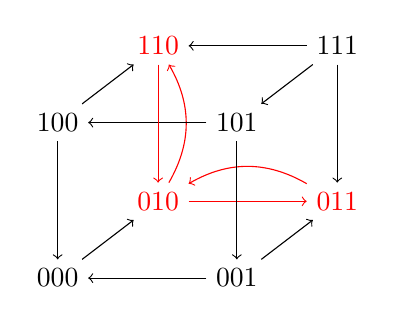
\begin{tikzpicture}[node distance=0.5cm and 0.5cm, every node/.style={scale=1.0}]
      \node[] (0) [] {000};
      \node[] (1) [right=of 0, xshift=1cm] {001};
      \node[red] (2) [above right=of 0] {010};
      \node[red] (3) [right=of 2, xshift=1cm] {011};
      \node[] (4) [above=of 0, yshift=1cm] {100};
      \node[] (5) [right=of 4, xshift=1cm] {101};
      \node[red] (6) [above=of 2, yshift=1cm] {110};
      \node[] (7) [above=of 3, yshift=1cm] {111};

      \draw[->] (0) edge [] (2);
      \draw[->] (1) edge [] (0);
      \draw[->] (1) edge [] (3);
      \draw[->, red] (2) edge [] (3);
      \draw[->, red] (2) edge [bend right] (6);
      \draw[->, red] (3) edge [bend right] (2);
      \draw[->] (4) edge [] (0);
      \draw[->] (4) edge [] (6);
      \draw[->] (5) edge [] (1);
      \draw[->] (5) edge [] (4);
      \draw[->, red] (6) edge [] (2);
      \draw[->] (7) edge [] (3);
      \draw[->] (7) edge [] (5);
      \draw[->] (7) edge [] (6);
    \end{tikzpicture}
  \end{column}
\end{columns}

\only<1>{
\hspace{0.8cm}

This BN has one min. trap space \(m = \{v_1 = \star, v_2 = \star, v_3 = \star\}\).
There is one attractor inside \(m\), \(\{010, 011, 110\}\).

\hspace{0.8cm}

The time-reversal BN has one max. trap space \(\{v_1 = 1, v_2 = \star, v_3 = 1\}\), which is self-negating.
Herein, \(\{\red{101}, 111\}\) is not in the attractor.

\hspace{0.8cm}

Applying the approach of mtsNFVS with \(U^-_{min} = \{v_1, v_3\}\) and \(b_1 = 1, b_3 = 1\).
Then, \(F = \{011, 110, 101\}\).
We can exclude \(\red{101}\) from \(F\) before any further analysis.
}

\only<2>{
\begin{block}{Theorem}
Let \(m\) be a trap space of a BN \(N\). Let \(N_m\) be the BN induced by \(m\) and \(N'\) be the time-reversal BN of \(N_m\). If \(s\) is an attractor state inside \(m\), then \(s\) cannot lie in any self-negating max. trap space of \(N'\).
\end{block}

\begin{block}{Proof}
Assume \(s\) is in a self-negating max. trap space \(M\) of \(N'\). Then, all states of the attractor containing \(s\) are also in \(M\). The states satisfy \(M\) but following the transitions of \(N\), they should reach states not satisfying \(M\) because \(M\) is a self-negating max. trap space of \(N'\). This is a contradiction.
\end{block}

}
\end{frame}

\begin{frame}
\frametitle{Reachability analysis}

We may still need to check the reachability in some cases, for example, there is a motif-avoidant attractor, the Preprocessing SSF is not good enough.

\hspace{0.8cm}

The reachability analysis is the \red{last resort} ensuring the correctness of our approach.

\hspace{0.8cm}

The reachability in ABNs is PSPACE-complete.
Its research is far from our focus now.
Hence, we should use the existing methods for the reachability analysis in a \blue{wise manner} relying on the information we have already known.

\end{frame}

\begin{frame}
\frametitle{Reachability analysis (cont.)}

For example, in the motif-avoidant attractor checking,
\begin{itemize}
  \item If \(|F| = 1\), it is likely that there is a motif-avoidant attractor, the result of the reachability analysis is likely unreachable. In this case, we should \blue{first use} a static analyzer (e.g., PINT~\cite{Pint}) that is efficient for very large models in the case of unreachable.
\end{itemize}

\hspace{0.0cm}

For example, in the process of each min. trap space \(m\),
\begin{itemize}
  \item If \(|F_m| = 2\), it is likely that there is only one attractor and the result of the reachability analysis is always reachable. In this case, we should \blue{first use} a bounded model checking-based approach (e.g., SAT, ASP) that is efficient for very large models in the case of reachable. Goal-driven Petri net unfolding~\cite{Chatain2016} is also a possible option in this case, but I do not think it can handle very large models.
\end{itemize}

\hspace{0.0cm}

We need to consider this problem thoroughly.

\end{frame}

\begin{frame}
\frametitle{Implementation}

% We need to alter the code of pystablemotifs in deep.

% \hspace{0.8cm}

% The first thing needed to be done may be to integrate Trappist~\footnote{\url{https://github.com/soli/trap-spaces-as-siphons}} to pystablemotifs.
% Since Trappist is written in Python, the integration should be easy.

% \hspace{0.8cm}

% We will discuss more about other implementation tasks.

Trappist (in Python): .bnet file \(\xrightarrow{pyeda}\) BDDs of Boolean functions \(\xrightarrow{}\) Petri net (digraph) \(\xrightarrow{}\) ASP (string) \(\xrightarrow{clingo}\) min./max. trap spaces (json)

\hspace{0.8cm}

We think that we should start from scratch, i.e., we remove completely the dependency on PyBoolNet because it uses a heavy data structure (i.e, prime-implicants).

\hspace{0.8cm}

We propose to design \red{a completely new system} for attractor detection and control.
We will gradually adapt the functions from pystablemotifs, mtsNFVS, and Trappist to the new system.
Of course, we need a \blue{good system design} first.

\hspace{0.8cm}

Note that our proposed approach contains many \blue{constituent tasks} (e.g., computation of min./max. trap spaces, computation of LDOI, driver node identification).
The new system should be easy to replace new implementations for each constituent task.

\end{frame}

\begin{frame}
\frametitle{Trappist: new features}

Now, Trappist supports computing
\begin{itemize}
  \item max. trap spaces \red{(original/time-reversal BN)}
  \item min. trap spaces \red{(original/time-reversal BN)}
  \item fixed points \red{(original/time-reversal BN)}
\end{itemize}

\hspace{0.8cm}

Introduction \dots

\end{frame}

\begin{frame}
\frametitle{System design}

Design a new system for attractor detection and control (input/output formats, components, functions, etc.).

\hspace{0.8cm}

Discuss \dots

\end{frame}

\begin{frame}
\frametitle{Computing negative feedback vertex sets}

Regarding \underline{the NFVS size}, the result of AEON is \blue{better} than that of mtsNFVS is most cases for real-world models. This is \red{opposite} for the case of random models.

\hspace{0.8cm}

Regarding \underline{the running time}, AEON is much faster than mtsNFVS for both real-world and random models.

\hspace{0.8cm}

There is a \red{matter} needed to be considered in our whole algorithm. If we only compute the NFVS (for the original ABN) one time, we can try both AEON and mtsNFVS. But, if we compute an NFVS for each intermediate ABN (induced in a maximal trap space or stable motif), we should try only AEON because of its time efficiency.

\hspace{0.8cm}

Of course, we can try all options and see which is the best. 

\end{frame}

\begin{frame}
\frametitle{Computing negative feedback vertex sets (cont.)}

``I think I have discovered the cause of the check failure. On line 62 of \texttt{SignedGraph.py}, there is the line \dots''

\hspace{0.8cm}

Indeed, \texttt{SignedGraph.py} is my own code (not of the FVSpython code).
Note that the FVSpython code only computes an FVS, not an NFVS.
Hence, I think the FVSpython code was properly converted from python 2 to python 3.

\hspace{0.8cm}

Now, the easiest option is that I will fix my own code so that it is properly compliant with python 3.

\end{frame}

\begin{frame}[fragile,allowframebreaks]
\frametitle{Compute the candidate set of states}

I first recall that the candidate set of states is the set of fixed points of the reduced STG with respect to an NFVS and a set of Boolean values assigned to nodes in this NFVS.

\hspace{0cm}

In our new algorithm, we restrict it to the terminal restriction space.
Specifically, we can ignore states belonging:
\begin{itemize}
  \item Stable motifs of \(G\): already in form of sub-spaces.
  \item Self-negating stable motifs of \(TR(G)\): already in form of sub-spaces.
  \item States for which \(R(X)\) is zero: needed to convert to a list of sub-spaces.
\end{itemize}

\hspace{0cm}

Actually, we only need to find the DNF of \(\neg R(X)\).
The computation of prime implicants is \blue{not necessary}.
There are two cases:
\begin{itemize}
  \item \(\neg R(X)\) is represented by a BDD: the union of all paths from the root to the one node. Each path is represented as a sub-space.
  \item \(\neg R(X)\) is represented by an expression (e.g., pyeda expr): each conjunction of the DNF is represented as a sub-space. As I know, the DNF conversion of pyeda does not require the computation of prime implicants.
\end{itemize}

\hspace{0cm}

Samuel: Since \(R(X)\) depends on the Boolean update functions, can we encode the avoidance of states in \(\neg R(X)\) directly in the encoded ASP (i.e., no need a DNF)?

\hspace{0cm}

Giang: It is possible. Let consider for example \(\neg R(X) = ((A \lor B) \land \neg C) \lor D\). Then the encoded ASP using the characterization of deadlocks should be:

\begin{verbatim*}
:- pD.
:- temp1 ; nC.
temp1 :- pA.
temp2 :- pB.
\end{verbatim*}

This ASP has the same set of answer sets (maybe not equivalent to) as the ASP using the DNF of \(\neg R(X)\) (i.e., \((A \land \neg C) \lor (B \land \neg C) \lor D\)) as follows:

\begin{verbatim*}
:- pD.
:- pA ; nC.
:- pB ; nC.
\end{verbatim*}

Note that in general obtaining a single DNF may be exponential.
The above approach does not required the DNF of \(\neg R(X)\), it only relies on the syntax of \(\neg R(X)\).

\hspace{0cm}

In addition, the \(\texttt{compute\_fixed\_point\_reduced\_STG}\) function should be included a new parameter \(\texttt{induced\_sub\_space}\), which ensures that all fixed points are inside a given maximal trap space.
Note however that this is needed if we only use the NFVS of the original ABN.

\end{frame}

\begin{frame}
\frametitle{Motif-avoidant checking}

``I highlighted a few minor style issues, plus a question about one of the functions in \texttt{state\_utils.py} \dots''

\hspace{0cm}

I assume that for a state, the value of every node is specified.
But of course, for the case that we do not specify all the values of the regulators of \(f\), an exception should be thrown.

\hspace{0cm}

I will fix it and other minor style issues.

\end{frame}

\begin{frame}
\frametitle{Next steps}

I propose to start writing the manuscript in parallel with the
implementation. 
We have four people and I think this strategy will help us to save a lot of time.

\hspace{0cm}

\underline{Publication plan}: is it similar to the case of the stable motifs-based method?
\begin{enumerate}
  \item A main journal paper: do you have any target in mind?
  \item A tool paper: Application notes in Oxford Bioinformatics?
\end{enumerate}

\hspace{0cm}

What do you think?

\end{frame}

\begin{frame}
\frametitle{A new related paper}

I have just found a related paper.

Sugyun An, So-Yeong Jang, Sang-Min Park, Chun-Kyung Lee, Hoon-Min Kim, Kwang-Hyun Cho, \emph{Global stabilizing control of large-scale biomolecular regulatory networks}, Bioinformatics, 2023;, btad045

\hspace{0cm}

It is compared to pystablemotifs for the target control.

\hspace{0cm}

I have not read the details yet. But for me, again the results reported in this paper seem not to be reliable because:

\begin{itemize}
  \item ``Among the biological Boolean networks in the Cell Collective (Helikar, et al., 2012), we selected 39 networks that have more than two attractors (including at least one point attractor) when all input nodes are fixed with the Off state.''
  \item From Fig 6.C, I found that it omits the \texttt{inflammatory-bowel} model (in the Cell Collective). This model has 47 nodes, and it is hard for PyBoolnet.
\end{itemize}

\end{frame}


\begin{frame}
\frametitle{Experimentation}

We plan to test the new method on models without \red{constant} nodes.

\hspace{0.8cm}

\red{N-K models}: expected to handle networks with \(K = 2\) and up to 500 nodes.

\hspace{0.8cm}

\red{scale-free models}: expected to handle networks with \(K = 10\) and up to 5000 nodes.

\hspace{0.8cm}

\red{real-world models}: expected to handle all the largest and most complex networks that we can find in the literature. The repository~\footnote{\url{https://github.com/sybila/biodivine-boolean-models}} maintained by Samuel Pastva is a good source.

\end{frame}

\begin{frame}
\frametitle{Conclusion}

The new approach exploits advantages of both pystablemotifs and mtsNFVS.

\hspace{0.8cm}

It benefits not only the attractor detection issue but also the control issue of asynchronous Boolean networks.

\hspace{0.8cm}

We believe that it will be the \blue{most promising} approach that can reach the genome scale.

\end{frame}

\begin{frame}
\frametitle{Collaboration}

We hope we will have a nice collaboration on this work.
Hence, we should make clear something at the beginning.

\hspace{0.8cm}

Participants:
\begin{itemize}
  \item Our side: Van-Giang Trinh and Samuel Pastva.
  \item Your side: Jordan Rozum and Kyu Hyong Park.
\end{itemize}

\hspace{0.8cm}

Authorship (if we can publish some papers :)): 
\begin{itemize}
  \item Two first authors, one from our side and one from your side with the equal contribution?
\end{itemize}

\hspace{0.8cm}

What do you think?

\end{frame}

\begin{frame}
\frametitle{Next steps}

\red{Task 1: Complete our new approach and make it as detailed as possible.}
\begin{itemize}
  \item Find solutions for some hard problems (e.g., the case of very huge attractors).
  \item Prepare more specific slides (or a report) presenting technical details of the new approach.
  \item Add more concrete examples for illustration.
\end{itemize}

\hspace{0.8cm}

\red{Task 2: Start the implementation of our new approach.}
\begin{itemize}
  \item Design a new system for attractor detection and control (input/output formats, components, functions, etc.).
  \item Programming
\end{itemize}

\hspace{0.8cm}

We should create a Github repository first.
Everything will be updated there.
\end{frame}

\begin{frame}
\frametitle{Our proposal}

I and Samuel will focus on Task 1.
Of course, Jordan and Kyu will also involve in this task to make the new approach as powerful as possible.

\hspace{0.8cm}

Jordan and Kyu will lead Task 2 because you already had the holistic view about pystablemotifs.
You can divide and assign to all of them implementation sub-tasks.
I and Samuel will contribute to this process.

\hspace{0.8cm}

Should keep regular exchanges between us.

\hspace{0.8cm}

Your suggestions?

\end{frame}

\begin{frame}
	\frametitle{New direction: network reduction}
	
	\only<1>{New preprint for enumerating attractors in asynchronous BNs based on reduction\footnote{Tonello, E., \& Paulevé, L. (2023). Attractor identification in asynchronous Boolean dynamics with network reduction. arXiv preprint arXiv:2305.01327.}.
	
	\hspace{0.8cm}
	
	\begin{block}{}
		Let \(\mathcal{A}\) be an \red{ABN} and \(w\) be its \blue{non-auto-regulated node}. Let \(\mathcal{A}^w\) be the ABN obtained by removing \(w\) from \(\mathcal{A}\) and replacing \(w\) by its Boolean function in all Boolean functions of its inputs. Then if \(att\) is an attractor of \(\mathcal{A}\), then there exists at least \blue{one attractor for \(\mathcal{A}^w\) in \(\pi^w(att)\)} and for each \(x \in \pi^w(att)\) contained in an attractor of \(\mathcal{A}^w\), \blue{\(\gamma^w(x) \in att\)}.
	\end{block}
	}
	\only<1>{
		\(\pi^w \colon \{0, 1\}^n \mapsto \{0, 1\}^{n - 1}\) is the \red{projection} on \(V \setminus \{w\}\).
		
		\hspace{0.8cm}
		
		\(\gamma^w \colon \{0, 1\}^{n- 1} \mapsto \{0, 1\}^{n}\) is the \red{mapping} where \(\gamma^w(x^w) = (x^w, f_w(x^w))\).
		
		\hspace{0.8cm}
		
		\blue{Can be used to efficiently enumerating all attractors of the original ABN.}
	}

	\only<2>{
		Some \red{issues}:
		\begin{itemize}
			\item \(\mathcal{A}^w\) may have \red{motif-avoidant} attractors, whereas \(\mathcal{A}\) have no ones. See the case of \(h\) in Figure 1 of the paper.
			\item \(\mathcal{A}^w\) may have \red{non-univocal} attractors, whereas \(\mathcal{A}\) may have no ones. See the case of \(g\) in Figure 1 of the paper.
			\item \(\mathcal{A}^w\) has \blue{less nodes} than \(\mathcal{A}\) but its Boolean functions may be \red{much more complex}.
			\begin{itemize}
				\item The minimum NFVS of \(\mathcal{A}^w\) may be \red{larger} than that of \(\mathcal{A}\).
				\item Reduce the efficiency of trappist because the \red{density} of \(\mathcal{A}^w\) may be much larger than that of \(\mathcal{A}\).
				\item For AEON, if there are \red{many dependencies}, the BDDs will also have many internal dependencies which \red{increase size}.
			\end{itemize}
		\end{itemize}
	}

	\only<3>{
		The new method is \blue{very efficient} for real-world models, but \red{not} for N-K models. Why?
		\begin{itemize}
			\item By applying the \blue{mediator-node reduction} to the set of real-world models, we found that the reduced models are \blue{very easy} to analyze and their number of attractors is \blue{equal} to that of the original models.
			\item In addition, real-world models are \blue{quite sparse}, leading to the Boolean functions of the reduced models are not very complex.
			\item This is not the case for N-K models.
		\end{itemize}
	}

	\only<4>{
		What we can explore in this direction?
		\small
		\begin{itemize}
			\item Of course, we can get a \blue{much smaller} candidate set for nfvs-motifs by computing attractors of the reduced model. If lucky, we can \blue{avoid} some bottlenecks of nfvs-motifs, for example, a minimal trap space \(m\) has too many free variables.
			\item Try to handle the problems of introducing \red{motif-avoidant} and \red{non-univocal} attractors to the reduced model.
			\item Heuristics for stop conditions and the order of removed nodes (based on not only the number of nodes but also the function complexity). I guess it might be related to \blue{FVS or NFVS}.
			\item Investigate how does the reduction change the structure of the succession diagram. For example, I guess \(\mathcal{A}^w\) might have a deeper SD than \(\mathcal{A}\) has.
			\item In case we must check reachability, how the reduction can help the \red{reachability analysis} more efficient?
			\item Investigate how the reduction can help the \red{control algorithms}.
			\item \red{Theoretical findings}
		\end{itemize}
	}

	\only<5>{
		\begin{block}{Conjecture}
			Let \(\mathcal{A}\) be an \red{ABN} and \(w\) be its \blue{mediator node}. Let \(\mathcal{A}^w\) be the ABN obtained by removing \(w\) from \(\mathcal{A}\) and replacing \(w\) by its Boolean function in all Boolean functions of its inputs. Then the set of attractors of \(\mathcal{A}^w\) \blue{one-to-one corresponds} to that of \(\mathcal{A}\).
		\end{block}
		\(w\) is a mediator node if \red{\(in(w) \cap out(w) \neq \emptyset\)}.
		
		\hspace{0cm}
		
		The case \blue{\(in(w) \cap out(w) \neq \emptyset \land \vert in(w)\vert = \vert out(w)\vert = 1\)} has been proven in\footnote{Saadatpour, A., Albert, R.,\& Reluga, T. C. (2013). A reduction method for Boolean network models proven to conserve attractors. SIAM Journal on Applied Dynamical Systems, 12(4), 1997-2011.}
		
		\hspace{0cm}
		
		Not sure whether the conjecture has been proven?
	}

	\only<6>{
		\begin{block}{Conjecture}
			Let \(\mathcal{A}\) be an \red{ABN} and \(w\) be its \blue{non-auto-regulated node}. Let \(\mathcal{A}^w\) be the ABN obtained by removing \(w\) from \(\mathcal{A}\) and replacing \(w\) by its Boolean function in all Boolean functions of its inputs. Then if \(m\) is a minimal trap space of \(\mathcal{A}\), then \(\pi^w(m)\) is also a minimal trap space of \(\mathcal{A}^w\).
		\end{block}
		
		\hspace{0cm}
		
		More generally, we can investigate the relations regarding trap spaces (minimal/maximal) between the reduced model and the original one.
	}

	\only<7>{
		I and Sam have discussed about this new direction. We also have some \blue{promising preliminary ideas}.
		
		\hspace{0cm}
		
		We propose us to consider this direction \red{after} finishing our first paper.
		
		\hspace{0cm}
		
		What do you think?
	}
	
\end{frame}

\section*{}
\begin{frame}
  \begin{center}
	  \Large{Thank you for your attention!}
	\end{center}
\end{frame}

\begin{frame}%[allowframebreaks]
\frametitle{Petri nets}
  \begin{columns}
    \begin{column}{0.4\textwidth}
      Bipartite graph
      
      \hspace{0.8cm}
      
      Places \(P\)
      
      Transitions \(T\)
      
      Weighted arcs \(W\)
    \end{column}
    \begin{column}{0.6\textwidth}
      \centering
        \scalebox{1.0}{
          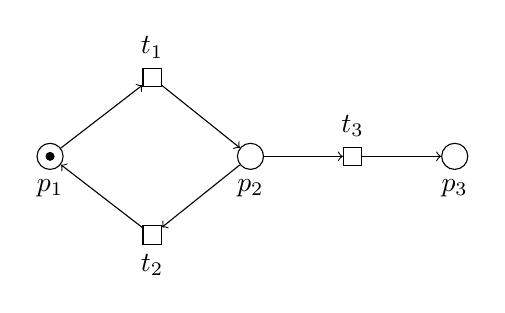
\begin{tikzpicture}[node distance=1cm and 1cm, every node/.style={scale=1.0}]
            \node[circle,draw,label=below:$p_1$] (p1) {};
            \node[circle,draw,fill=black,scale=0.3] (p1_0) {};
            \node[circle,draw,label=below:$p_2$] (p2) [right=of p1, xshift=1.2cm] {};
    
            \node[rectangle,draw,label=above:$t_1$] (t1) [right=of p1, yshift=1cm] {};
            \node[rectangle,draw,label=below:$t_2$] (t2) [right=of p1, yshift=-1cm] {};
            \node[rectangle,draw,label=above:$t_3$] (t3) [right=of p2] {};
    
            \node[circle,draw,label=below:$p_3$] (p3) [right=of t3] {};
            
            \draw[->] (p1) -- (t1);
            \draw[->] (t1) -- (p2);
            \draw[->] (p2) -- (t2);
            \draw[->] (t2) -- (p1);
            \draw[->] (p2) -- (t3);
            \draw[->] (t3) -- (p3);
          \end{tikzpicture}
        }
    \end{column}
  \end{columns}
  
  \hspace{0.8cm}
  
  A \emph{marking} for a Petri net is a mapping \(m : P \mapsto \mathbb{N}\) that assigns a number of tokens to each place.
  A place \(p\) is marked by a marking \(m\) if and only if \(m(p) > 0\). For example, \(p_1\) is marked, \(p_2\) and \(p_3\) are unmarked.
  
  \hspace{0.8cm}
  
  We shall write \(pred(x)\) (resp.\ \(succ(x)\)) to represent the set of vertices that have a (non-zero weighted) arc leading to (resp.\ coming from) \(x\). For example, \(pred(p_2) = \{t_1\}\), \(succ(p_2) = \{t_2, t_3\}\), \(pred(t_2) = \{p_2\}\), and \(succ(t_2) = \{p_1\}\).
  
\end{frame}

\begin{frame}%[allowframebreaks]
\frametitle{Siphons}

\begin{block}{Siphon}

  A \emph{siphon} of a Petri net \((P, T, W)\) is a set of places \(S\) such that:
  \[\forall t\in T, S\cap succ(t)\not =\emptyset\Rightarrow S\cap pred(t)\not =\emptyset.\]
  
\end{block}

\hspace{0.8cm}

Once a siphon is unmarked, it remains unmarked. 

\hspace{0.8cm}

\begin{columns}
    \begin{column}{0.5\textwidth}
      \(S = \{p_1, p_3\}\) is not a siphon because \(S \cap succ(t_3) = \{p_1, p_3\} \cap \{p_3\} = \{p_3\} \not =\emptyset\) but \(S \cap pred(t_3) = \{p_1, p_3\} \cap \{p_2\} = \emptyset\).
      
      \hspace{0.8cm}
      
      Here: \(\emptyset\), \(\{p_1, p_2\}\), \(\{p_1, p_2, p_3\}\)
    \end{column}
    \begin{column}{0.5\textwidth}
      \centering
        \scalebox{1.0}{
          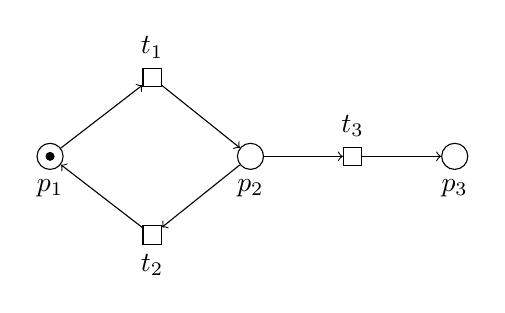
\begin{tikzpicture}[node distance=1cm and 1cm, every node/.style={scale=1.0}]
            \node[circle,draw,label=below:$p_1$] (p1) {};
            \node[circle,draw,fill=black,scale=0.3] (p1_0) {};
            \node[circle,draw,label=below:$p_2$] (p2) [right=of p1, xshift=1.2cm] {};
    
            \node[rectangle,draw,label=above:$t_1$] (t1) [right=of p1, yshift=1cm] {};
            \node[rectangle,draw,label=below:$t_2$] (t2) [right=of p1, yshift=-1cm] {};
            \node[rectangle,draw,label=above:$t_3$] (t3) [right=of p2] {};
    
            \node[circle,draw,label=below:$p_3$] (p3) [right=of t3] {};
            
            \draw[->] (p1) -- (t1);
            \draw[->] (t1) -- (p2);
            \draw[->] (p2) -- (t2);
            \draw[->] (t2) -- (p1);
            \draw[->] (p2) -- (t3);
            \draw[->] (t3) -- (p3);
          \end{tikzpicture}
        }
    \end{column}
\end{columns}
  
\end{frame}

\begin{frame}%[allowframebreaks]
\frametitle{Traps}

\begin{block}{Trap}

  A \emph{trap} of a Petri net \((P, T, W)\) is a set of places \(S\) such that:
  \[\forall t\in T, S\cap pred(t)\not =\emptyset\Rightarrow S\cap succ(t)\not =\emptyset.\]
  
\end{block}

\hspace{0.8cm}

Once a trap is marked (i.e., at least one of its places is marked), it remains marked.

\hspace{0.8cm}

\begin{columns}
    \begin{column}{0.5\textwidth}
      \(S = \{p_1, p_3\}\) is not a trap because \(S \cap pred(t_1) = \{p_1, p_3\} \cap \{p_1\} = \{p_1\} \not =\emptyset\) but \(S \cap succ(t_1) = \{p_1, p_3\} \cap \{p_2\} = \emptyset\).
      
      \hspace{0.8cm}
      
      Here: \(\emptyset\), \(\{p_1, p_2, p_3\}\)
    \end{column}
    \begin{column}{0.5\textwidth}
      \centering
        \scalebox{1.0}{
          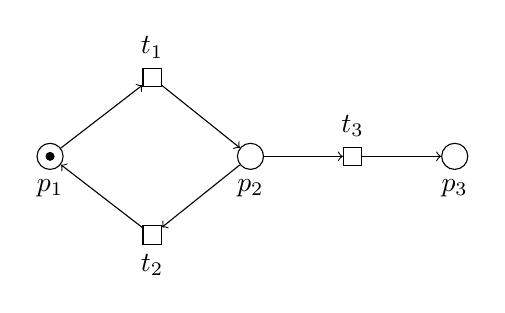
\begin{tikzpicture}[node distance=1cm and 1cm, every node/.style={scale=1.0}]
            \node[circle,draw,label=below:$p_1$] (p1) {};
            \node[circle,draw,fill=black,scale=0.3] (p1_0) {};
            \node[circle,draw,label=below:$p_2$] (p2) [right=of p1, xshift=1.2cm] {};
    
            \node[rectangle,draw,label=above:$t_1$] (t1) [right=of p1, yshift=1cm] {};
            \node[rectangle,draw,label=below:$t_2$] (t2) [right=of p1, yshift=-1cm] {};
            \node[rectangle,draw,label=above:$t_3$] (t3) [right=of p2] {};
    
            \node[circle,draw,label=below:$p_3$] (p3) [right=of t3] {};
            
            \draw[->] (p1) -- (t1);
            \draw[->] (t1) -- (p2);
            \draw[->] (p2) -- (t2);
            \draw[->] (t2) -- (p1);
            \draw[->] (p2) -- (t3);
            \draw[->] (t3) -- (p3);
          \end{tikzpicture}
        }
    \end{column}
\end{columns}
  
\end{frame}

\begin{frame}
  \frametitle{Petri net of a Boolean model}
  
The original encoding was established in~\cite{chaouiya2004qualitative}.

\hspace{0.8cm}

Two places for each gene: \(v \rightsquigarrow p_v, \overline{p_v}\)

\hspace{0.8cm}

Solutions of \(f_v \not \leftrightarrow v\) \(\rightsquigarrow\) transitions from \(p_v\) to \(\overline{p_v}\) (and back)

\hspace{0.8cm}

At any marking \(m\) of the Petri net encoding a Boolean model, it always holds that \(m(p_v) + m(\overline{p}_v) = 1\).

\begin{columns}
  \begin{column}{0.4\textwidth}
    \begin{equation*}
      \begin{cases}
        f_1 = (x_1 \land x_2) \lor (\neg x_1 \land \neg x_2)\\
        f_2 = (x_1 \land x_2) \lor (\neg x_1 \land \neg x_2)\\
      \end{cases}
    \end{equation*}
  \end{column}
    \begin{column}{0.6\textwidth}
    \centering
        \scalebox{1.0}{
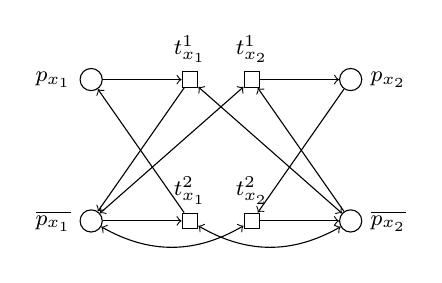
\begin{tikzpicture}[node distance=1cm and 1cm, every node/.style={scale=1.0}]\footnotesize
  \node[circle,draw,label=left:$p_{x_1}$] (x1) {};
  \node[circle,draw,label=left:$\overline{p_{x_1}}$] (nx1) [below=of x1, yshift=-0.5cm] {};
    
  \node[circle,draw,label=right:$p_{x_2}$] (x2) [right=of x1, xshift=2.0cm] {};
  \node[circle,draw,label=right:$\overline{p_{x_2}}$] (nx2) [below=of x2, yshift=-0.5cm] {};
    
  \node[rectangle,draw,label=above:$t^1_{x_1}$] (t1x1) [right=of x1] {};
  \node[rectangle,draw,label=above:$t^2_{x_1}$] (t2x1) [right=of nx1] {};
  
  \node[rectangle,draw,label=above:$t^1_{x_2}$] (t1x2) [left=of x2] {};
  \node[rectangle,draw,label=above:$t^2_{x_2}$] (t2x2) [left=of nx2] {};
  
  \draw[->] (x1) -- (t1x1);
  \draw[->] (t1x1) -- (nx1);
  \draw[<->] (t1x1) -- (nx2);
  
  \draw[->] (nx1) -- (t2x1);
  \draw[->] (t2x1) -- (x1);
  \draw[<->] (t2x1) edge [bend right] (nx2);
  
  \draw[->] (x2) -- (t2x2);
  \draw[->] (t2x2) -- (nx2);
  \draw[<->] (t2x2) edge [bend left] (nx1);
  
  \draw[->] (nx2) -- (t1x2);
  \draw[->] (t1x2) -- (x2);
  \draw[<->] (t1x2) -- (nx1);
\end{tikzpicture}
        }
    \end{column}
\end{columns}

\hspace{0.8cm}

\end{frame}

\begin{frame}
\frametitle{Conflict-free siphons/traps}

A siphon/trap is called \textbf{conflict-free} if it does not contain both \(p_v\) and \(\overline{p_v}\) for all \(v \in V\).

\hspace{0.8cm}

\begin{columns}
    \begin{column}{0.5\textwidth}
    \centering
        \scalebox{1.0}{
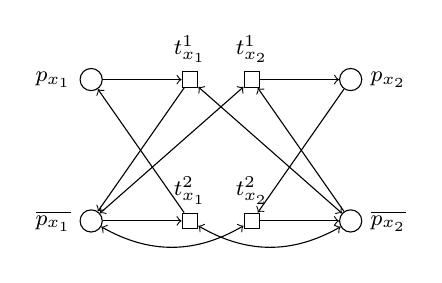
\begin{tikzpicture}[node distance=1cm and 1cm, every node/.style={scale=1.0}]\footnotesize
  \node[circle,draw,label=left:$p_{x_1}$] (x1) {};
  \node[circle,draw,label=left:$\overline{p_{x_1}}$] (nx1) [below=of x1, yshift=-0.5cm] {};
    
  \node[circle,draw,label=right:$p_{x_2}$] (x2) [right=of x1, xshift=2.0cm] {};
  \node[circle,draw,label=right:$\overline{p_{x_2}}$] (nx2) [below=of x2, yshift=-0.5cm] {};
    
  \node[rectangle,draw,label=above:$t^1_{x_1}$] (t1x1) [right=of x1] {};
  \node[rectangle,draw,label=above:$t^2_{x_1}$] (t2x1) [right=of nx1] {};
  
  \node[rectangle,draw,label=above:$t^1_{x_2}$] (t1x2) [left=of x2] {};
  \node[rectangle,draw,label=above:$t^2_{x_2}$] (t2x2) [left=of nx2] {};
  
  \draw[->] (x1) -- (t1x1);
  \draw[->] (t1x1) -- (nx1);
  \draw[<->] (t1x1) -- (nx2);
  
  \draw[->] (nx1) -- (t2x1);
  \draw[->] (t2x1) -- (x1);
  \draw[<->] (t2x1) edge [bend right] (nx2);
  
  \draw[->] (x2) -- (t2x2);
  \draw[->] (t2x2) -- (nx2);
  \draw[<->] (t2x2) edge [bend left] (nx1);
  
  \draw[->] (nx2) -- (t1x2);
  \draw[->] (t1x2) -- (x2);
  \draw[<->] (t1x2) -- (nx1);
\end{tikzpicture}
        }
    \end{column}
  \begin{column}{0.5\textwidth}
    \begin{tabular}{ll}
      \toprule
      Siphon & Conflict-free? \\ \midrule
      \red{\(\emptyset\)} & \red{yes} \\
      \red{\(\{\overline{p_{x_1}}, \overline{p_{x_2}}\}\)} & \red{yes} \\
      \(\{p_{x_1}, \overline{p_{x_1}}\}\) & no \\
      \(\{p_{x_2}, \overline{p_{x_2}}\}\) & no \\
      \bottomrule
    \end{tabular}
  \end{column}
\end{columns}

\hspace{0.8cm}

A conflict-free siphon (resp. trap) is \emph{maximal} if it is not a subset of any other conflict-free siphon (resp. trap).

\end{frame}

\begin{frame}
\frametitle{Conflict-free siphons are trap spaces}

\begin{block}{Theorem 1}

  Let \(\mathcal{M}\) be a Boolean model and \(\mathcal{P}\) be its Petri net encoding. There is a \blue{one-to-one correspondence} between the set of \textbf{trap spaces} of \(\mathcal{M}\) and the set of \textbf{conflict-free siphons} of \(\mathcal{P}\).
  
\end{block}

\begin{columns}
  \begin{column}{0.4\textwidth}
    \begin{equation*}
      \begin{cases}
        f_1 = (x_1 \land x_2) \lor (\neg x_1 \land \neg x_2)\\
        f_2 = (x_1 \land x_2) \lor (\neg x_1 \land \neg x_2)\\
      \end{cases}
    \end{equation*}
  \end{column}
    \begin{column}{0.6\textwidth}
    \centering
        \scalebox{1.0}{
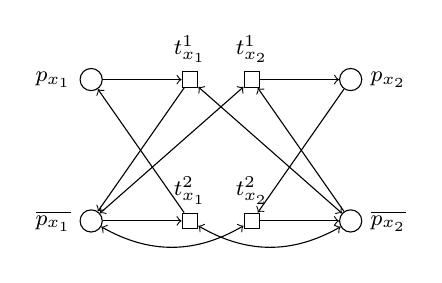
\begin{tikzpicture}[node distance=1cm and 1cm, every node/.style={scale=1.0}]\footnotesize
  \node[circle,draw,label=left:$p_{x_1}$] (x1) {};
  \node[circle,draw,label=left:$\overline{p_{x_1}}$] (nx1) [below=of x1, yshift=-0.5cm] {};
    
  \node[circle,draw,label=right:$p_{x_2}$] (x2) [right=of x1, xshift=2.0cm] {};
  \node[circle,draw,label=right:$\overline{p_{x_2}}$] (nx2) [below=of x2, yshift=-0.5cm] {};
    
  \node[rectangle,draw,label=above:$t^1_{x_1}$] (t1x1) [right=of x1] {};
  \node[rectangle,draw,label=above:$t^2_{x_1}$] (t2x1) [right=of nx1] {};
  
  \node[rectangle,draw,label=above:$t^1_{x_2}$] (t1x2) [left=of x2] {};
  \node[rectangle,draw,label=above:$t^2_{x_2}$] (t2x2) [left=of nx2] {};
  
  \draw[->] (x1) -- (t1x1);
  \draw[->] (t1x1) -- (nx1);
  \draw[<->] (t1x1) -- (nx2);
  
  \draw[->] (nx1) -- (t2x1);
  \draw[->] (t2x1) -- (x1);
  \draw[<->] (t2x1) edge [bend right] (nx2);
  
  \draw[->] (x2) -- (t2x2);
  \draw[->] (t2x2) -- (nx2);
  \draw[<->] (t2x2) edge [bend left] (nx1);
  
  \draw[->] (nx2) -- (t1x2);
  \draw[->] (t1x2) -- (x2);
  \draw[<->] (t1x2) -- (nx1);
\end{tikzpicture}
        }
    \end{column}
\end{columns}

\begin{tabular}{ll}
  \toprule
  Trap space & Conflict-free siphon \\ \midrule
  \(\star\star\) & \(\emptyset\) \\
  11 & \(\{\overline{p_{x_1}}, \overline{p_{x_2}}\}\) \\
  \bottomrule
\end{tabular}

\end{frame}

\begin{frame}
\frametitle{Maximal conflict-free siphons are minimal trap spaces}

\begin{block}{Theorem 2}

  Let \(\mathcal{M}\) be a Boolean model and \(\mathcal{P}\) be its Petri net encoding. There is a \blue{one-to-one correspondence} between the set of \textbf{minimal trap spaces} of \(\mathcal{M}\) and the set of \textbf{maximal conflict-free siphons} of \(\mathcal{P}\).
  
\end{block}

\begin{columns}
  \begin{column}{0.4\textwidth}
    \begin{equation*}
      \begin{cases}
        f_1 = (x_1 \land x_2) \lor (\neg x_1 \land \neg x_2)\\
        f_2 = (x_1 \land x_2) \lor (\neg x_1 \land \neg x_2)\\
      \end{cases}
    \end{equation*}
  \end{column}
    \begin{column}{0.6\textwidth}
    \centering
        \scalebox{1.0}{
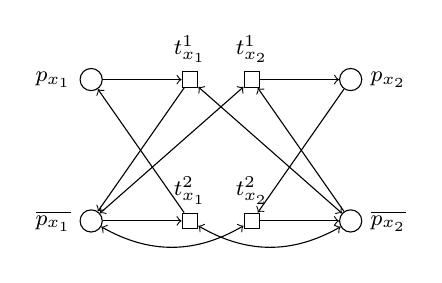
\begin{tikzpicture}[node distance=1cm and 1cm, every node/.style={scale=1.0}]\footnotesize
  \node[circle,draw,label=left:$p_{x_1}$] (x1) {};
  \node[circle,draw,label=left:$\overline{p_{x_1}}$] (nx1) [below=of x1, yshift=-0.5cm] {};
    
  \node[circle,draw,label=right:$p_{x_2}$] (x2) [right=of x1, xshift=2.0cm] {};
  \node[circle,draw,label=right:$\overline{p_{x_2}}$] (nx2) [below=of x2, yshift=-0.5cm] {};
    
  \node[rectangle,draw,label=above:$t^1_{x_1}$] (t1x1) [right=of x1] {};
  \node[rectangle,draw,label=above:$t^2_{x_1}$] (t2x1) [right=of nx1] {};
  
  \node[rectangle,draw,label=above:$t^1_{x_2}$] (t1x2) [left=of x2] {};
  \node[rectangle,draw,label=above:$t^2_{x_2}$] (t2x2) [left=of nx2] {};
  
  \draw[->] (x1) -- (t1x1);
  \draw[->] (t1x1) -- (nx1);
  \draw[<->] (t1x1) -- (nx2);
  
  \draw[->] (nx1) -- (t2x1);
  \draw[->] (t2x1) -- (x1);
  \draw[<->] (t2x1) edge [bend right] (nx2);
  
  \draw[->] (x2) -- (t2x2);
  \draw[->] (t2x2) -- (nx2);
  \draw[<->] (t2x2) edge [bend left] (nx1);
  
  \draw[->] (nx2) -- (t1x2);
  \draw[->] (t1x2) -- (x2);
  \draw[<->] (t1x2) -- (nx1);
\end{tikzpicture}
        }
    \end{column}
\end{columns}

\begin{tabular}{ll}
  \toprule
  Trap space & Conflict-free siphon \\ \midrule
  \(\star\star\) & \(\emptyset\) \\
  \red{11} & \red{\(\{\overline{p_{x_1}}, \overline{p_{x_2}}\}\)} \\
  \bottomrule
\end{tabular}

\end{frame}

\begin{frame}
\frametitle{Proposed method for minimal trap space computation}

From Theorem 2, we propose a new method for computing minimal trap spaces of a Boolean model \(\mathcal{M}\).
\begin{itemize}
  \item Build the Petri net encoding \(\mathcal{P}\) of \(\mathcal{M}\).
  \item Compute all maximal conflict-free siphons of \(\mathcal{P}\).
  \item Convert the obtained maximal conflict-free siphons into the corresponding minimal trap spaces.
\end{itemize}
\end{frame}

\begin{frame}
\frametitle{Petri net transformation}

Transforming a Boolean model into its Petri net encoding can be done via computing Disjunctive Normal Forms (DNF) of each Boolean function~\cite{chatain2014characterization}. This transformation is implemented in the bioLQM\footnote{\url{http://www.colomoto.org/biolqm/}} library using BDDs.

\hspace{0.8cm}

Though this might appear quite computationally intensive it is important to remark first that contrary to the prime-implicants case, there is no need to find \emph{minimal} DNFs.

\hspace{0.8cm}

We use the above transformation in our proposed method.

\end{frame}

\begin{frame}
\frametitle{Maximal conflict-free siphon computation}

Characterize all siphons of the encoded Petri net as a system of Boolean rules.
\begin{equation*}
\label{eq:siphon}
p \in S \Rightarrow \bigvee_{p' \in pred(t)}p' \in S, p \in P, t \in T, t \in pred(p)
\end{equation*}

Add to the system the Boolean rules representing the conflict-freeness.
\begin{equation*}
\label{eq:conflict}
p_v \in S \Rightarrow \overline{p_v} \not \in S \wedge \overline{p_v} \in S \Rightarrow p_v \not \in S, v \in V
\end{equation*}

Encode the system as an ASP.

\hspace{0.8cm}

Use an ASP solver (e.g., clingo~\cite{DBLP:journals/aicom/GebserKKOSS11}) to compute all set-inclusion maximal answer sets of the ASP.

\hspace{0.8cm}

Set-maximality through “heuristics”

\texttt{clingo --heuristic=Domain --enum-mod=domRec --dom-mod=3}

\end{frame}

% \section*{References}
\begin{frame}[allowframebreaks]
  %\small
  \frametitle{References}
	%\bibliographystyle{unsrt}
	%\bibliographystyle{alpha}
	\bibliographystyle{apalike}
	\bibliography{ref}
\end{frame}

\end{document}